\documentclass[12pt, titlepage]{article}

\usepackage{longtable}
\usepackage[utf8]{inputenc}
\usepackage{fullpage}
\usepackage{amsmath, mathtools}
\usepackage{amsfonts}
\usepackage{amssymb}
\usepackage{graphicx}
\usepackage{colortbl}
\usepackage{xr}
\usepackage{xr-hyper}
\usepackage{hyperref}
\usepackage{longtable}
\usepackage{xfrac}
\usepackage{tabularx}
\usepackage{float}
\usepackage{siunitx}
\usepackage{booktabs}
\usepackage{caption}
\usepackage{pdflscape}
\usepackage{fixltx2e}
\usepackage{afterpage}
\usepackage{seqsplit}
\usepackage{underscore}
\usepackage{lscape}
\usepackage[english]{babel}
\usepackage[T1]{fontenc}
\usepackage{booktabs}
\usepackage{tabularx}
\usepackage{hyperref}
\usepackage{nameref}
\usepackage{enumitem}


% checklist
\newlist{todolist}{itemize}{3}
\setlist[todolist]{label=$\square$}


\hypersetup{
    colorlinks,
    citecolor=blue,
    filecolor=black,
    linkcolor=red,
    urlcolor=blue
}
\usepackage[round]{natbib}
\MakeRobust{\ref}% avoid expanding it when in a textual label

\makeatletter
\newcommand{\labeltext}[2]{%
  \@bsphack
  \csname phantomsection\endcsname % in case hyperref is used
  \def\@currentlabel{#1}{\label{#2}}%
  \@esphack
}
%% Comments

\usepackage{color}

\newif\ifcomments\commentstrue %displays comments
%\newif\ifcomments\commentsfalse %so that comments do not display

\ifcomments
\newcommand{\authornote}[3]{\textcolor{#1}{[#3 ---#2]}}
\newcommand{\todo}[1]{\textcolor{red}{[TODO: #1]}}
\else
\newcommand{\authornote}[3]{}
\newcommand{\todo}[1]{}
\fi

\newcommand{\wss}[1]{\authornote{blue}{SS}{#1}} 
\newcommand{\plt}[1]{\authornote{magenta}{TPLT}{#1}} %For explanation of the template
\newcommand{\an}[1]{\authornote{cyan}{Author}{#1}}

%% Common Parts

\newcommand{\progname}{Mechatronics Engineering} % PUT YOUR PROGRAM NAME HERE
\newcommand{\authname}{Team \# 34, ParkingLotHawk
\\ Fady Zekry Hanna, zekryhf
\\ Winnie Trandinh, trandint
\\ Muhammad Ali, alim102
\\ Muhammad Khan, khanm120} % AUTHOR NAMES                  

\usepackage{hyperref}
    \hypersetup{colorlinks=true, linkcolor=blue, citecolor=blue, filecolor=blue,
                urlcolor=blue, unicode=false}
    \urlstyle{same}
                                

%\externaldocument[]{SRS}
\externaldocument{../SRS/SRS}

%%\documentclass{article}
\usepackage[utf8]{inputenc}
\usepackage{fullpage}
\usepackage{amsmath, mathtools}
\usepackage{amsfonts}
\usepackage{amssymb}
\usepackage{graphicx}
\usepackage{colortbl}
\usepackage{xr}
\usepackage{hyperref}
\usepackage{longtable}
\usepackage{xfrac}
\usepackage{tabularx}
\usepackage{float}
\usepackage{siunitx}
\usepackage{booktabs}
\usepackage{caption}
\usepackage{pdflscape}
\usepackage{afterpage}
\usepackage{seqsplit}
\usepackage{underscore}
\usepackage{lscape}
\usepackage[english]{babel}
\usepackage[T1]{fontenc}


% For easy change of table widths
\newcommand{\colZwidth}{1.0\textwidth}
\newcommand{\colAwidth}{0.13\textwidth}
\newcommand{\colBwidth}{0.82\textwidth}
\newcommand{\colCwidth}{0.1\textwidth}
\newcommand{\colDwidth}{0.05\textwidth}
\newcommand{\colEwidth}{0.8\textwidth}
\newcommand{\colFwidth}{0.17\textwidth}
\newcommand{\colGwidth}{0.5\textwidth}
\newcommand{\colHwidth}{0.28\textwidth}


\newcommand{\deftheory}[9][Not Applicable]
{
\newpage
\noindent \rule{\textwidth}{0.5mm}

\paragraph{RefName: } \textbf{#2} \phantomsection 
\label{#2}

\paragraph{Label:} #3

\noindent \rule{\textwidth}{0.5mm}

\paragraph{Equation:}

#4

\paragraph{Description:}

#5

\paragraph{Notes:}

#6

\paragraph{Source:}

#7

\paragraph{Ref.\ By:}

#8

\paragraph{Preconditions for \hyperref[#2]{#2}:}
\label{#2_precond}

#9

\paragraph{Derivation for \hyperref[#2]{#2}:}
\label{#2_deriv}

#1

\noindent \rule{\textwidth}{0.5mm}

}

\begin{document}

\title{
Software Requirements Specification for ParkingLotHawk \\
  \large MECHTRON 4TB6 Capstone Design Project 
    }

\author{\authname Team \#34 \\
Fady Zekry Hanna, zekryhf \\
Winnie Trandinh, trandint \\
Muhammad Ali, alim102 \\
Muhammad Khan, khanm120}

\date{\today}
	
\maketitle

~\newpage

\pagenumbering{roman}

\tableofcontents

~\newpage

\section*{Revision History}

\begin{tabularx}{\textwidth}{p{3cm}p{2cm}X} 
\toprule {\bf Date} & {\bf Version} & {\bf Notes}\\
\midrule
Oct 5, 2022 & 1.0 & Team Finalized SRS\\

\bottomrule
\end{tabularx}

~\newpage

\pagenumbering{arabic}

\section{Introduction}
\label{sec:Intro}
\subsection{Purpose}
The purpose of the project will be to design an aerial drone, called ParkingLotHawk, that can detect how many parking spots are available in any given parking lot. ParkingLotHawk can be operated by property personnel to communicate to drivers on how many spots are available at a parking lot. ParkingLotHawk will explore over any parking lot designated by the user and will aggregate visual information and output the amount of parking spots available. Many parking lots today do not have this data and this data can be used for many reasons. The data can be used by retailers to know how long customers stay at specific stores or location. This data can also be used for drivers to know if there are parking spots available in a specific location allowing for drivers to not waste time and resources in a full parking lot. 
\subsection{Scope}
The product specified in this SRS \ref{DefTable} is about an autonomous aerial drone for helping parking lot operators understand the state of their parking lot. The product specified does not require the operator to manually control or move the drone, rather the requirement describes various autonomous flight modes. The specified drone shall support the ability to both create a path to reach its specified location, as well as create and follow a path to explore large parking lot sections autonomously. During flight, the specified drone shall transmit live information about the parking lot sections it detects. The completed product, a combination of the physical drone and any equipment/application intended to be kept by the parking lot operator to communicate with the drone, is called the ParkingLotHawk. A solution that implements the requirements will help parking lot authorities of outdoor lots quickly gain valuable information without requiring permanent solution, large monetary and time investments, or complex training. 



\subsection{Definitions, Acronyms, and Abbreviations}

\begin{table}[!h]
\begin{center}
\caption {Key terms, acronyms, and abbreviations are defined.} 
\label{DefTable}
\begin{tabular}{ | m{3cm} | m{11cm} | }
\hline
Term & Definition. \\
\hline
Inclement Weather & Weather with rain, snow, fog, and/or winds over 50 km/hour. \\
\hline
Parking Lot Authorities & Event organizers for whome parking lot management is one of thier tasks. Examples include property managers, and concert organizers.  \\
\hline
Parking Lot Operator (Operator) & Person responsible for managing the product during operation. \\
\hline
Clear Boundaries & The border surrounding the parking lot. For example the border between the lot and sidewalks, buildings, curbs, and sections of grass.\\
\hline
Flight Controller & The central part of the drone that receives most sensor input and is responsible for controlling the propellers.\\
\hline
Flight States & The states of the state machine that require the drone to be aerially flying, detailed in the requirements \ref{flightModes}.\\
\hline
PC & Personal Computer. \\
\hline
MVP & Minimum Viable Product. \\
\hline
SRS & Software Requirement Specifications. \\
\hline
\end{tabular}
\end{center}
\end{table}

\subsection{References}
There are no external software documents referenced in the SRS. 

\subsection{Overview}
The SRS is organized to follow the IEEE 1998 template. \nameref{sec:Intro} contains the purpose of the SRS as well as the scope of the product and the problem it solves. \nameref{sec:Desc}  refines the scope of the product further. It provides more detail about the products environment, primary functions, intended users, constraints, and finally assumptions. \nameref{sec:Req} contains a detailed description of all requirements, organized into sections for readability. Finally, the \nameref{appendix} contains \nameref{appendixa} regarding new knowledge and skills the team needs to create the specified product, along with approaches to how the team will acquire the knowledge. The \nameref{appendixb}  also contains the formal transition tables between the states of the finite state machine which will be later introduced within \nameref{subsec:ProdFunc}.
\section{Overall Description}
\label{sec:Desc}
General factors that affect the product and the requirements are described in the following subsections. A high-level overview of the product functions are also described (see \nameref{subsec:ProdFunc}). 
\subsection{Product Perspective}
The system specified is an independent and stand-alone parking lot tool. It does not fit into or interface with a larger system of parking lot and security technologies the operator may have available. 

The environment consists of an outdoor parking lot and the operator's PC. The operator's PC shall be operating with Windows 10 or Windows 11.

\subsection{Product Functions}
\label{subsec:ProdFunc}
This subsection describes the behaviour overview of the ParkingLotHawk by splitting its functionality into various interconnected states of operation. These states are shown within the \nameref{InfFSM} and are further refined within \nameref{sec:funcReqs}. 
\subsubsection{Idle State}
\label{Idle State}
The product is powered on and communicating with the operator application, but all motors are turned off. 
\subsubsection{Hover State}
\label{Hover State}
The product maintains its current longitudinal and latitudinal position, and hovers at a pre-defined operator selected height. 
\subsubsection{Manual Location Move State}
\label{Manual Location Move State}
The product shall move to an operator specified location, and hover at a pre-defined operator selected height. Note that this height does not need to be the same as the height specified in the Hover State. 
\subsubsection{Autonomous Explore State}
\label{Autonomous Explore State}
The product shall autonomously explore within the current parking lot without operator input. 
\subsubsection{Configure State}
\label{Configure State}
During this state, the operator is able to define parameters of operation that are not configurable in other states. 
\subsubsection{Off State}
\label{Off State}
The product shall be unpowered and stops communication with the operator application. 
\subsubsection{Land State}
\label{Land State}
The product shall land at its initial launch location.
\subsubsection{Desired Location Error State}
\label{Desired Location Error State}
This error state occurs when the operator specifies an invalid desired position and shall provide the appropriate error message to the operator. 
\subsubsection{No Parking Lot Detected Error State}
\label{No Parking Lot Detected Error State}
This error state occurs when the product does not detect a valid parking lot, and shall provide the appropriate error message to the operator.
\subsubsection{Malfunction State}
\label{Malfunction State}
This error state occurs when an internal/external malfunction occurs in such a way that nominal performance is not possible. The resulting action by the product will be further specified within \nameref{sec:funcReqs}. 

The normal modes of operation include the following:
\begin{itemize}
  \item Idle State
  \item Hover State
  \item Manual Location Move State
  \item Autonomous Explore State
  \item Configure State
  \item Off State
\end{itemize}
The flight modes of operation \label{flightModes} include the following:
\begin{itemize}
  \item Hover State
  \item Manual Location Move State
  \item Autonomous Explore State
   \item No Parking Lot Detected Error State
   \item Desired Location Out of Bounds Error State
\end{itemize}
With the exception of the Configure State and Off State, the product shall update continuously update c_CurrentView and c_OccupancyMap for the operator. These requirements are further refined within \nameref{sec:funcReqs}. 

The error modes are listed below:
\begin{itemize}
    \item Desired Location Error State
    \item No Parking Lot Detected Error State
    \item Malfunction State
\end{itemize}
These modes are used to handle errors either from the operator, or internally from the product. 

The behaviour overview of the product is described below, with each directional arrow representing a transition between states:
\begin{figure}[h!]
  \begin{center} 
  \caption{Informal Finite State Machine Diagram } 
  \label{InfFSM}
 
        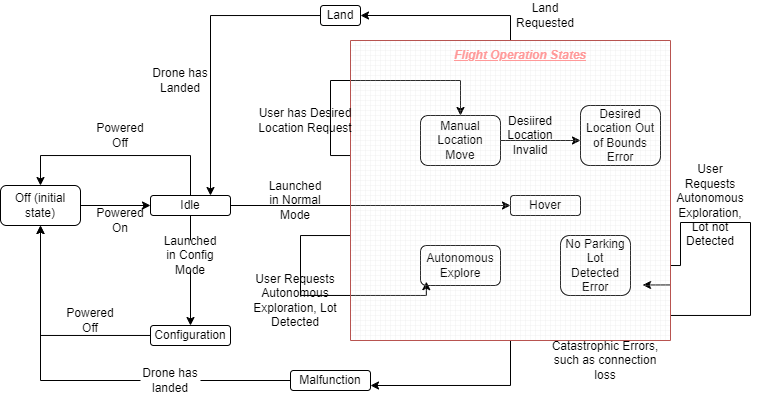
\includegraphics[width=0.5\textwidth]{InformalFSM.png}
  \end{center}
\end{figure}

\subsection{User characteristics}
The stakeholders are Dr. Spencer Smith, the MECHTRON 4TB6 teaching assistants, parking lot authorities \ref{DefTable}, parking lot operators, and visitors of the parking lot. All demographics mentioned would find the data of the ParkingLotHawk useful. There is no technical or software knowledge expected for users of the ParkingLotHawk. The user will need to turn the drone on and place it close to a parking lot.  The ParkingLotHawk is made mindful of the society and community and its health impacts; therefore, little to no air or noise pollution shall occur, and no invasion of privacy shall ensue.
\subsection{Constraints}
\label{sec:Constraints}
The purpose of the system is to provide parking lot information to parking lot operators, who in turn could use that information to decrease the amount of time visitors spend to find a parking spot. As the user can come from a non-technical background, the constraints on the usability of the product should be considered. If the system chooses to use radio communication between the operator's laptop and the product, it must abide by national radio frequency regulations of 2.4MHz. Furthermore, radio communication can only work within approximately 2 km from one point to the other while still abiding by the national regulations. The project constraint present is a maximum budget of \$ 750.  Canadian regulatory policy does not allow for drone flight within 1 nautical mile (about 2 km) from heliports and 3 nautical miles (5.6 km) from airports\cite{canada_flying_2020}. If the drone weighs over 25 kg, the team will need to get special permission from Transport Canada before flying the drone\cite{canada_find_2021}; therefore, the product should be under a weight of 25kg to support widespread adoption.
\subsection{Assumptions}
\label{sec:Assumptions}
The assumptions of the project are:
\begin{itemize}

  \item Operator does not fly the drone exceeding a specified amount of time.
  \item Birds do not interfere with the drone.
  \item Operator's PC has a Windows 10 or 11 OS.
  \item Parking lot lines are visible to the naked eye.
  \item Operation done under non-inclement weather\ref{DefTable}. 

\end{itemize}

\subsection{Apportioning of Requirements}
The Phase in Plan is composed of three main releases:  
\begin{itemize}
    \item Phase I: Proof of Concept - November 14, 2022
    \item Phase II: Revision 0 (Minimal Viable Product (MVP) ) - February 6, 2023 
    \item Phase III: Revision 1 - March 27, 2023
\end{itemize}
Each requirement will then be assigned to one of these phases within \nameref{sec:Req}, indicated by their Phase. 

\section{Specific requirements }
\label{sec:Req}
This section of the SRS contains all requirements of the product in order to further refine the scope of the product.

\subsection{External Interfaces}
Input Variables: Input variables are set/configured before any flight operations are entered \ref{flightModes} . They are constant throughout the drones flight operation \ref{flightModes} .


\begin{figure}[!h]
  \begin{center} 
  \caption{System Context Diagram} 
 
        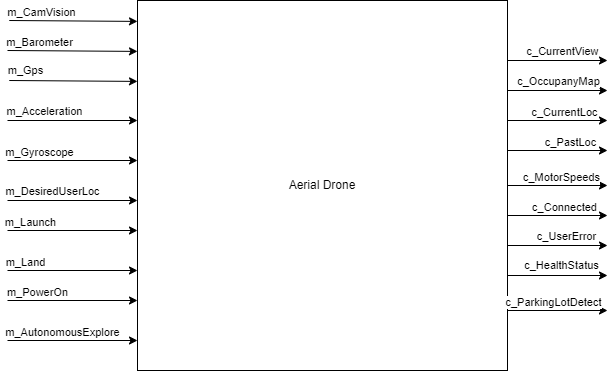
\includegraphics[width=0.5\textwidth]{ContextDiagram.png}
  \end{center}
\end{figure}



\begin{table}[!h]
\begin{center}
\caption {Input Variables} \label{tab:title}
\label{InputVariables}
\begin{tabular}{ | m{3cm} | m{2cm} | m{2cm} | m{6cm} | } 
\hline
 Variable Name & Type & Unit & Description \\ 
 \hline
i\_Mode & Enumeration & 	0 - Normal, 1 - Configure &	Set by the user to choose whether they want to configure internal parameters or if they want regular operation. \\
\hline i\_MinHoverHeight & float	&m	& Minimum aerial hover height set by user\\
\hline i\_MaxHoverHeight & float	&m	& Maximum aerial hover height set by user\\
\hline i\_DesiredHoverHeight & float	&m	& Desired aerial hover height set by user\\
\hline 
\end{tabular}
\end{center}
\end{table}

\newpage
Monitored Variables are variables that are continuously monitored by the product.
\begin{table}[!h]
\begin{center}
\caption {Monitored Variables} \label{tab:title}
\begin{tabular}{ | m{3cm} | m{2cm} | m{2cm} | m{6cm} | } 
\hline
 Variable Name & Type & Unit & Description \\ 
 \hline
m\_Acceleration	& Vector& m/s^2 & three-dimensional vector containing acceleration relative to frame of the drone. \\
\hline
m\_Gyroscope & Vector	&Rad &	 three-dimensional vector containing orientation relative to frame of the drone.\\
\hline
m\_Gps	& Tuple &	 GPS coordinates (degrees-minutes-seconds (DMS), height (m))&	 current GPS coordinates of the drone with height in the second tuple.\\
\hline
m\_Barometer	& Float&	atm	 &Altitude detection using atmospheric pressure measurement\\
\hline
m\_DesiredUserLoc &	GPS Location&	 GPS coordinates (DMS) &	 Desired location of the aerial drone set by user.\\
\hline
m\_Launch &	Boolean	 &  - &	Indicates if the operator desires the drone to begin operation and turn on all peripherals.  \\
\hline
m\_AutonomousExplore &	Boolean &	 -	 &Indicates if the operator desires the drone to autonomously explore the parking lot.\\ 
\hline
m\_PowerOn&	Boolean  &	- &	Indicates if the operator desires the drone to be On or Off.\\
\hline
m\_Land&Boolean&	-&	Indicates if the operator desires the drone to land.\\
\hline
 m\_CamVision &	Image&	Array of Pixels&	Latest image of the section of the parking lot currently visible to the drone.\\
\hline

\end{tabular}
\end{center}
\end{table}

\newpage

Controlled Variables are variables that are outputted by the system. Some are visible to the operator on their application, while others help to indirectly accomplish functional requirements. 

\begin{table}[!h]
\begin{center}
\caption {Controlled Variables} \label{tab:title}
\begin{tabular}{ | m{3cm} | m{2cm} | m{2cm} | m{6cm} |}
\hline
 Variable Name & Type & Unit & Description \\ 
 \hline
 c\_CurrentView &	Image &	Array of Pixels &	Live visual display of parking lot section the drone's currently sees, as well as any further annotations and text.\\
 \hline
c\_OccupancyMap &	Image &	Array of Pixels &	Map of available parking spots based on the drone’s previous paths. \\
\hline
c\_CurrentLoc & 	Tuple&	\{GPS coordinates (DMS) , height (m)\} & GPS coordinates are stored at the first index, height is stored in the second index.	Estimated longitudinal coordinate, lateral coordinate and height of the drone.\\
\hline
c\_PastLoc&	Vector &	1/ Degrees, minutes, and seconds (DMS)&	Trace of the drone's location in the past 60 seconds (vector of GPS locations).\\
\hline
c\_MotorSpeeds &Vector&	   rad/s^2 &	 n-dimensional vector containing the motor speeds of however many motors the drone chooses to use (2 for helicopter, 4 for quadcopter, 6 for hexcopter, etc.). The vector contains speeds of each motor clockwise from front of the drone.\\

\hline

c\_Connected & Boolean &	- &	Indicates if connection between the drone and the operator's application is established\\
\hline
c\_ParkingLotDetected&	Boolean &	-&	Indicated if a parking lot is detected in the c_CurrentView.\\
\hline
c\_UserError &	Enumeration &	0 - None,
1 - Desired_Location_Out_Of_Bounds,
2 - No_Lot_Detected_State&	Indicates if a command the user requested is not feasible.\\
\hline
c\_HealthStatus &	Enumeration &	0 - Healthy,
1 - Unhealthy&	Indicates if the drone's mechanical and electrical state allows it to safely fly.  For example if there is mechanical damage, the value should be Unhealthy.\\
\hline
\end{tabular}
\end{center}
\end{table}





\newpage

\subsection{Functional Requirements}
\label{sec:funcReqs}
The following requirements are required in order to achieve the product's functions, as stated in \nameref{subsec:ProdFunc}.

\subsubsection{General Functional Requirements}

\begin{table}[!h]
\begin{center}
\caption {GEN\_001} 
\label{GEN_001}
\begin{tabular}{ | m{3cm} | m{11cm} | }
\hline
Description & The product shall be able to recognize Clear Boundaries \ref{DefTable}. This requirement is a refinement of the \nameref{Autonomous Explore State}. \\
\hline
Rationale & This requirement ensures that the product is able to implement basic autonomy, such as not traveling past the parking lot boundaries. \\
\hline
Phase & II \\
\hline
Likely to Change & No. This requirement is required to implement the \nameref{Autonomous Explore State}. \\
\hline
Associated Inputs and Outputs & m\_CamVision. \\
\hline
\end{tabular}
\end{center}
\end{table}


\begin{table}[!h]
\begin{center}
\caption {GEN\_002} 
\label{GEN_002}
\begin{tabular}{ | m{3cm} | m{11cm} | } 
\hline
Description & The product shall provide live update of c\_CurrentLoc, c\_CurrentView and c\_OccupancyMap during all normal and non-configurational operation states. This requirement is a refinement of the normal and non-configuration operation states specified in Section \ref{subsec:ProdFunc}. \\
\hline
Rationale & This requirement ensures that the product always provides the latest controlled variable information to the operator. \\
\hline
Phase & II \\
\hline
Likely to Change & No. This requirement is a part of the MVP and must be present to make the product achieve its product functions. \\
\hline
Associated Inputs and Outputs & m\_CamVision, c\_CurrentLoc, c\_CurrentView, and c\_OccupancyMap. \\
\hline
\end{tabular}
\end{center}
\end{table}

\begin{table}[!h]
\begin{center}
\caption {GEN\_003} 
\label{GEN_003}
\begin{tabular}{ | m{3cm} | m{11cm} | } 
\hline
Description & The product shall allow the operator to configure the i\_MinHoverHeight, i\_MaxHoverHeight, and i\_DesiredHoverHeight. This requirement is a refinement of the \nameref{Configure State}. \\
\hline
Rationale & The value of these parameters depends on the operators view preferences and parking lot conditions. For example a parking lot with a lot of large trucks may be better suited to higher hovering heights. \\
\hline
Phase & I \\
\hline
Likely to Change & No. This requirement is vital to the operation of the product, as it must be suited to different parking lot environments. \\
\hline
Associated Inputs and Outputs & i\_MinHoverHeight, i\_MaxHoverHeight, and i\_DesiredHoverHeight. \\
\hline
\end{tabular}
\end{center}
\end{table}

\begin{table}[!h]
\begin{center}
\caption {GEN\_004} 
\label{GEN_004}
\begin{tabular}{ | m{3cm} | m{11cm} | } 
\hline
Description & The condition i\_MinHoverHeight <= i\_DesiredHoverHeight <= i\_MaxHoverHeight shall always be true. This requirement is a refinement of the \nameref{Configure State}. \\
\hline
Rationale & This requirement ensures logical values for the parameters are set by the operator. \\
\hline
Phase & I \\
\hline
Likely to Change & No. This requirement is required to check the inputted values by the operator. \\
\hline
Associated Inputs and Outputs & i\_MinHoverHeight, i\_DesiredHoverHeight, and i\_MaxHoverHeight. \\
\hline
\end{tabular}
\end{center}
\end{table}

\begin{table}[!h]
\begin{center}
\caption {GEN\_005} 
\label{GEN_005}
\begin{tabular}{ | m{3cm} | m{11cm} |}
\hline
Description & The product shall be able to identify non-occupied parking spots. This requirement is a refinement of the normal and non-configuration operation states specified in Section \ref{subsec:ProdFunc}. \\
\hline
Rationale & This requirement ensures that the product is able to create the occupancy map. \\
\hline
Phase & III \\
\hline
Likely to Change & No. This requirement is required to create the occupancy map (c_OccupancyMap), which is one of the main functions of the product during the Phase III Release. \\
\hline
Associated Inputs and Outputs & m\_CamVision, c\_ParkingLotDetected, and c\_OccupancyMap. \\
\hline
\end{tabular}
\end{center}
\end{table}

\begin{table}[!h]
\begin{center}
\caption {GEN\_006} 
\label{GEN_006}
\begin{tabular}{ | m{3cm} | m{11cm} | }
\hline
Description & The product shall be shall highlight non-occupied parking slots on the operator's display (update c_CurrentView). This requirement is a refinement of the normal and non-configuration operation states specified in Section \ref{subsec:ProdFunc}. \\
\hline
Rationale & This requirement ensures that the product is able to create the occupancy map. \\
\hline
Phase & III \\
\hline
Likely to Change & No. This requirement is a key feature of the occupancy map in order to efficiently communicate the data to the operator. \\
\hline
Associated Inputs and Outputs & m\_CamVision, c\_CurrentView, c\_ParkingLotDetected, and c\_OccupancyMap. \\
\hline
\end{tabular}
\end{center}
\end{table}

\clearpage
\newpage

\subsubsection{State Implementation Requirements}
\label{sec:stateReqs}

\begin{table}[!h]
\begin{center}
\caption {STA\_000} 
\label{STA_000}
\begin{tabular}{ | m{3cm} | m{11cm} | } 

\hline
Description & The product shall implement an Idle state. During this state, the solution is powered on but motors are stationary. This requirement is a refinement of the \nameref{Idle State}, and further refined by \nameref{PERF_007}, \nameref{SAFE_001}, \nameref{SAFE_003}, and \nameref{USE_003}. \\
\hline
Rationale & This state is used to ensure that the operator can safely hold the drone and access the mechanical switch that controls m\_PowerOn. \\
\hline
Phase & I \\
\hline
Likely to Change & No. This requirement is required for the safety of the operator. \\
\hline
Associated Inputs and Outputs & m\_PowerOn and c\_Connected. \\
\hline
\end{tabular}
\end{center}
\end{table}

\begin{table}[!h]
\begin{center}
\caption {STA\_001} 
\label{STA_001}
\begin{tabular}{ | m{3cm} | m{11cm} | }
\hline
Description & The product shall implement a Hover State. During this state, the solution shall fly and hover to height i\_MaxHoverHeight. The drone shall keep the same lateral location it is currently at.  This requirement is a refinement of the \nameref{Hover State} and is further refined by \nameref{PERF_002}, \nameref{PERF_004}, \nameref{PERF_005}, \nameref{PERF_006}, \nameref{PERF_007}, \nameref{SAFE_001}, \nameref{SAFE_003}, and \nameref{USE_003}. \\
\hline
Rationale & This state is used for when the product is waiting for further operator commands. Hover height is selected to be i\_MaxHoverHeight, so that the drone can see as much of the parking lot section as it can. This makes the transition to \nameref{Autonomous Explore State} more likely. \\
\hline
Phase & II \\
\hline
Likely to Change & No. This requirement is a key feature of the MVP, and is required in order to gather any useful information to the operator. \\
\hline
Associated Inputs and Outputs & m\_Barometer, m\_Acceleration, m\_Gyroscope, m\_Gps, i\_MaxHoverHeight, and c\_MotorSpeeds. \\
\hline
\end{tabular}
\end{center}
\end{table}

\begin{table}[!h]
\begin{center}
\caption {STA\_002} 
\label{STA_002}
\begin{tabular}{ | m{3cm} | m{11cm} | }
\hline
Description & The product shall implement a Manual Location Move State. During this state, the drone moves to the m\_DesiredUserLoc, and hovers at that location with height i\_DesiredHoverHeight. This requirement is a refinement of the \nameref{Manual Location Move State} and is further refined by \nameref{PERF_003}, \nameref{PERF_004}, \nameref{PERF_006}, \nameref{PERF_007}, \nameref{SAFE_001}, \nameref{SAFE_003}, and \nameref{USE_003}. \\
\hline
Rationale & This state is used for when the the product needs to provide the operator the ability to move the drone to a specific location. \\
\hline
Phase & II \\
\hline
Likely to Change & No. This requirement is a key feature of the product, and is required in order for the operator to make changes to the product's path. \\
\hline
Associated Inputs and Outputs & m\_DesiredUserLoc, m\_Barometer, m\_Acceleration, m\_Gyroscope, m\_Gps, i\_DesiredHoverHeight, and c\_MotorSpeeds. \\
\hline
\end{tabular}
\end{center}
\end{table}

\begin{table}[!h]
\begin{center}
\caption {STA\_003} 
\label{STA_003}
\begin{tabular}{ | m{3cm} | m{11cm} | }
\hline
Description & The product shall implement an Autonomous Explore State. During this state the drone will create its own path to explore and remain within the parking lot it currently detects. This requirement is a refinement of the \nameref{Autonomous Explore State} and is further refined by \nameref{PERF_001}, \nameref{PERF_004}, \nameref{PERF_007}, \nameref{SAFE_001}, \nameref{SAFE_003}, and \nameref{USE_003}. \\
\hline
Rationale & This state is used for when the operator does not need to constantly instruct the drone to move. \\
\hline
Phase & III \\
\hline
Likely to Change & No. This requirement is an important part of the Phase III Release, as it allows for automated creation of the occupancy map. \\
\hline
Associated Inputs and Outputs & m\_Barometer, m\_Acceleration, m\_Gyroscope, m\_Gps, m\_AutonomouseExplore, m\_CamVision, c\_CurrentView, and c\_MotorSpeeds. \\
\hline
\end{tabular}
\end{center}
\end{table}

\begin{table}[!h]
\begin{center}
\caption {STA\_004} 
\label{STA_004}
\begin{tabular}{ | m{3cm} | m{11cm} | }
\hline
Description & The product shall implement a Configure state. During this state settings and parameters that cannot be changed during flight can be changed. The Input Variables i\_MinHoverHeight, i\_MaxHoverHeight and i\_DesiredHoverHeight can be changed in this state. The product is powered on but motors are stationary. This requirement is a refinement of the \nameref{Configure State}, and references \nameref{GEN_003}. This is further refined by \nameref{PERF_004}, \nameref{PERF_007}, \nameref{SAFE_001}, \nameref{SAFE_003}, and \nameref{USE_003}. \\
\hline
Rationale & This state is used to allow parameters that are unsafe to change during flight operation, to be safely changed through a special process. During this state the operator can safely hold the drone. Such parameters are outlined in \nameref{InputVariables}. \\
\hline
Phase & II \\
\hline
Likely to Change & No. This requirement is required to ensure safety of the operator, as well as the product from unsafe changes during operation. \\
\hline
Associated Inputs and Outputs & i\_Mode, i\_MinHoverHeight, i\_MaxHoverHeight, and i\_DesiredHoverHeight. \\
\hline
\end{tabular}
\end{center}
\end{table}

\begin{table}[!h]
\begin{center}
\caption {STA\_005} 
\label{STA_005}
\begin{tabular}{ | m{3cm} | m{11cm} | }
\hline
Description & The product shall implement an Off state.  All modules are powered off. No battery power is consumer. c\_UserError is set to None, c\_HealthStatus is set to Unhealthy, and c\_Connected is set to false. All values in the matrices c\_MotorSpeeds, c\PastLoc, c\_OccupancyMap, and c\_CurrentView are set to 0. This requirement is a refinement of the \nameref{Off State} and is further refined by \nameref{PERF_004}, \nameref{PERF_007}, \nameref{SAFE_001}, and \nameref{SAFE_003} \\
\hline
Rationale & This state is used to explicitly state what it means for the drone to be off. \\
\hline
Phase & I \\
\hline
Likely to Change & No. This requirement is required for the safe operation, transport, and handling of the product. \\
\hline
Associated Inputs and Outputs & c\_UserError, c\_HealthStatus, c\_Connected, c\_MotorSpeeds, c\PastLoc, c\_OccupancyMap, and c\_CurrentView. \\
\hline
\end{tabular}
\end{center}
\end{table}

\begin{table}[!h]
\begin{center}
\caption {STA\_006} 
\label{STA_006}
\begin{tabular}{ | m{3cm} | m{11cm} | }
\hline
Description & The product shall implement a Land state. In the land state the solution first travel laterally to the initial launch location, and then lands vertically downward. Once physically landed, the drone enters the Idle state. This requirement is a refinement of the \nameref{Land State} and is further refined by \nameref{PERF_002}, \nameref{PERF_004}, \nameref{PERF_006}, \nameref{PERF_007}, \nameref{SAFE_001}, \nameref{SAFE_003}, and \nameref{USE_003}. \\
\hline
Rationale & This state is used to explicitly designate a landing path and command. \\
\hline
Phase & II \\
\hline
Likely to Change & No. This requirement is required for stopping the operation of the product. \\
\hline
Associated Inputs and Outputs & m\_Barometer, m\_Acceleration, m\_Gyroscope, m\_Gps, and c\_MotorSpeeds. \\
\hline
\end{tabular}
\end{center}
\end{table}

\begin{table}[!h]
\begin{center}
\caption {STA\_007} 
\label{STA_007}
\begin{tabular}{ | m{3cm} | m{11cm} | }
\hline
Description & The product shall implement an Desired Location Error state. Upon entry to this state, the c\_UserError variable is set to Desired_Location_Out_Of_Bounds. The drone proceeds to Hover at its current location. Upon exit of this state, the drone shall set c\_UserError to None. This requirement is a refinement of the \nameref{Desired Location Error State} and is further refined by \nameref{PERF_007}, \nameref{SAFE_001}, \nameref{SAFE_003}, and \nameref{USE_003}. \\
\hline
Rationale & This state is used to indicate explicitly that the operator's request cannot be met.  \\
\hline
Phase & II \\
\hline
Likely to Change & No. This requirement is required for clear communication with the operator to handle unsupported requests. \\
\hline
Associated Inputs and Outputs & m\_Barometer, m\_Acceleration, m\_Gyroscope, m\_Gps, c\_UserError, and c\_MotorSpeeds. \\
\hline
\end{tabular}
\end{center}
\end{table}

\begin{table}[!h]
\begin{center}
\caption {STA\_008} 
\label{STA_008}
\begin{tabular}{ | m{3cm} | m{11cm} | }
\hline
Description & The product shall implement a No Parking Lot Detected Error state. Upon entry to this state, the c\_UserError variable is set to No_Lot_Detected_State. The drone proceeds to Hover at its current location. Upon exit of this state, the drone shall set c\_UserError to None. This requirement is a refinement of the \nameref{No Parking Lot Detected Error State} and is further refined by \nameref{PERF_007}, \nameref{SAFE_001}, \nameref{SAFE_003}, and \nameref{USE_003}. \\
\hline
Rationale & This state is used to indicate explicitly that the product cannot detect a parking lot. \\
\hline
Phase & II \\
\hline
Likely to Change & No. This requirement is required for clear communication with the operator to handle unsupported requests. \\
\hline
Associated Inputs and Outputs & m\_Barometer, m\_Acceleration, m\_Gyroscope, m\_Gps, c\_UserError, and c\_MotorSpeeds. \\
\hline
\end{tabular}
\end{center}
\end{table}

\begin{table}[!h]
\begin{center}
\caption {STA\_009} 
\label{STA_009}
\begin{tabular}{ | m{3cm} | m{11cm} | }
\hline
Description & The product shall implement a Malfunction state. During this state the drone sets the c\_HealthStatus to Unhealthy. It then tries to land at its launch location, which if is not possible the drone instead lands vertically on the land below. After landing the drone enters the Off state. This requirement is a refinement of the \nameref{Malfunction State} and is further refined by \nameref{PERF_007}, \nameref{SAFE_001}, \nameref{SAFE_003}, and \nameref{USE_003}. \\
\hline
Rationale & This state is used to ensure that the product can handle large malfunctions that can occur during operation. \\
\hline
Phase & II \\
\hline
Likely to Change & No. This requirement is required to handle malfunctioning components during operation. \\
\hline
Associated Inputs and Outputs & m\_barometer, m\_acceleration, m\_gyroscope, m\_gps, c\_healthStatus, and c\_motorSpeed. \\
\hline
\end{tabular}
\end{center}
\end{table}

\clearpage
\newpage

\subsubsection{State Transition Requirements}
\label{transReqs}
The following requirements are refinements of all the states specified in Section \ref{sec:stateReqs}, and specifies the product's transitions between states. These requirements will not be changed unless the states are changed.

\begin{table}[!h]
\begin{center}
\caption {TRANS\_001} 
\label{TRANS_001}
\begin{tabular}{ | m{3cm} | m{11cm} | }
\hline
Description & Upon the m\_PowerOn becoming false, the drone shall enter the Off state. This requirement references the \nameref{Off State}. \\
\hline
Rationale & This requirement ensures that the product can turn off safely. \\
\hline
Phase & I \\
\hline
Associated Inputs and Outputs & m\_PowerOn. \\
\hline
\end{tabular}
\end{center}
\end{table}

\begin{table}[!h]
\begin{center}
\caption {TRANS\_002} 
\label{TRANS_002}
\begin{tabular}{ | m{3cm} | m{11cm} | }
\hline
Description & Upon the m\_PowerOn becoming true, the drone shall enter the Idle state. This requirement references the \nameref{Idle State} and the requirement \nameref{SAFE_005}. \\
\hline
Rationale & This requirement ensures that the propellers do not damage the operator after touching the m\_PowerOn switch.  \\
\hline
Phase & I \\
\hline
Associated Inputs and Outputs & m\_PowerOn. \\
\hline
\end{tabular}
\end{center}
\end{table}

\begin{table}[!h]
\begin{center}
\caption {TRANS\_003} 
\label{TRANS_003}
\begin{tabular}{ | m{3cm} | m{11cm} | }
\hline
Description & Upon the m\_Launch becoming true, the drone shall enter the Hover state if the i\_Mode was set to normal, and enters the Configure state if the i\_Mode was set to configure. This requirement references the \nameref{Hover State} and the \nameref{Configure State}. \\
\hline
Rationale & This requirement facilitates the setup and configuration of the product.  \\
\hline
Phase & II \\
\hline
Associated Inputs and Outputs & m\_Launch and i\_Mode. \\
\hline
\end{tabular}
\end{center}
\end{table}

\begin{table}[!h]
\begin{center}
\caption {TRANS\_004} 
\label{TRANS_004}
\begin{tabular}{ | m{3cm} | m{11cm} | }
\hline
Description & If in the Hover state, and c\_ParkingLotDetected is equal to true, the product shall enter the Autonomous Explore state and explore the detected lot. If two parking lots are detected at the same time, it arbitrarily picks one to explore. This requirement references the \nameref{Hover State} and the \nameref{Autonomous Explore State}. \\
\hline
Rationale & This requirement ensures that the default mode of operation is Autonomous Explore after entering the Hover state.  \\
\hline
Phase & III \\
\hline
Associated Inputs and Outputs & c\_ParkingLotDetected. \\
\hline
\end{tabular}
\end{center}
\end{table}

\begin{table}[!h]
\begin{center}
\caption {TRANS\_005} 
\label{TRANS_005}
\begin{tabular}{ | m{3cm} | m{11cm} | }
\hline
Description & Once the user enters or changes m\_DesiredUserLoc, the drone shall automatically enters the Manual Location Move state. This requirement references the \nameref{Manual Location Move State}. \\
\hline
Rationale & This requirement ensures that the product shall take the operator's request with higher priority than any other kind of operation. \\
\hline
Phase & II \\
\hline
Associated Inputs and Outputs & m\_DesiredUserLoc. \\
\hline
\end{tabular}
\end{center}
\end{table}

\begin{table}[!h]
\begin{center}
\caption {TRANS\_006} 
\label{TRANS_006}
\begin{tabular}{ | m{3cm} | m{11cm} | }
\hline
Description & If while in the Manual Location Hold state and the product determines that m\_DesiredUserLoc is outside parking lot boundaries, the product shall enter the Desired Location Error state. This requirement references the \nameref{Manual Location Move State} and the \nameref{Desired Location Error State}. \\
\hline
Rationale & This requirement ensures that the product shall notify any issues with the operator's request at the moment it is detected, so that the operator can make adjustments. \\
\hline
Phase & II \\
\hline
Associated Inputs and Outputs & m\_DesiredUserLoc. \\
\hline
\end{tabular}
\end{center}
\end{table}

\begin{table}[!h]
\begin{center}
\caption {TRANS\_007} 
\label{TRANS_007}
\begin{tabular}{ | m{3cm} | m{11cm} | }
\hline
Description & When m\_AutonomousExplore is set to true and c\_ParkingLotDetected is equal to true, the product shall enter the Autonomous Explore state. This requirement references the \nameref{Autonomous Explore State}. \\
\hline
Rationale & This requirement ensures that the product shall take the operator's request with higher priority than any other kind of operation. \\
\hline
Phase & II \\
\hline
Associated Inputs and Outputs & m\_AutonomousExplore and c\_ParkingLotDetected. \\
\hline
\end{tabular}
\end{center}
\end{table}

\begin{table}[!h]
\begin{center}
\caption {TRANS\_008} 
\label{TRANS_008}
\begin{tabular}{ | m{3cm} | m{11cm} | }
\hline
Description & When m\_AutonomousExplore is set to true but c\_ParkingLotDetected is equal to false, the product shall enter the No Parking Lot Detected Error state. This requirement references the \nameref{No Parking Lot Detected Error State}. \\
\hline
Rationale & This requirement ensures that the product shall notify any issues with the operator's request at the moment it is detected, so that the operator can make adjustments. \\
\hline
Phase & II \\
\hline
Associated Inputs and Outputs & m\_AutonomousExplore and c\_ParkingLotDetected. \\
\hline
\end{tabular}
\end{center}
\end{table}

\begin{table}[!h]
\begin{center}
\caption {TRANS\_009} 
\label{TRANS_009}
\begin{tabular}{ | m{3cm} | m{11cm} | }
\hline
Description & Upon m\_Land being true, the product shall enter the Land state. This requirement references the \nameref{Land State}. \\
\hline
Rationale & This requirement ensures that the product is able to land at the requested time. \\
\hline
Phase & II \\
\hline
Associated Inputs and Outputs & m\_Land. \\
\hline
\end{tabular}
\end{center}
\end{table}

\begin{table}[!h]
\begin{center}
\caption {TRANS\_010} 
\label{TRANS_010}
\begin{tabular}{ | m{3cm} | m{11cm} | }
\hline
Description & If c\_Connected becomes false for more than 5 seconds at any point during operation, then the product shall enter the Malfunction state. This requirement references the \nameref{Malfunction State}. \\
\hline
Rationale & This requirement ensures that the product detects connectivity errors, and is able to handle such occurrences. \\
\hline
Phase & I \\
\hline
Associated Inputs and Outputs & c\_Connected. \\
\hline
\end{tabular}
\end{center}
\end{table}


\begin{table}[!h]
\begin{center}
\caption {A tractability table linking non-functional requirements to the functional requirements they reference. If a requirement has no dependencies or relationships, then it is not mentioned. }
\label{TRACE_FR_NFR}
\begin{tabular}{ | m{7cm} | m{7cm} | }
\hline
Functional Requirement & Non-functional requirement  \\
\hline
\nameref{STA_000} & \nameref{PERF_007}, \nameref{SAFE_001}, \nameref{SAFE_003}, \nameref{USE_003}  \\
\hline
\nameref{STA_001} & \nameref{PERF_002}, \nameref{PERF_004}, \nameref{PERF_005}, \nameref{PERF_006}, \nameref{PERF_007}, \nameref{SAFE_001}, \nameref{SAFE_003}, \nameref{USE_003}  \\
\hline
\nameref{STA_002} & \nameref{PERF_003}, \nameref{PERF_004}, \nameref{PERF_006}, \nameref{PERF_007}, \nameref{SAFE_001}, \nameref{SAFE_003}, \nameref{USE_003}  \\
\hline
\nameref{STA_003} & \nameref{PERF_001}, \nameref{PERF_004}, \nameref{PERF_007}, \nameref{SAFE_001}, \nameref{SAFE_003}, \nameref{USE_003}  \\
\hline
\nameref{STA_004} & \nameref{PERF_004}, \nameref{PERF_007}, \nameref{SAFE_001}, \nameref{SAFE_003}, \nameref{USE_003}  \\
\hline
\nameref{STA_005} & \nameref{PERF_004}, \nameref{PERF_007}, \nameref{SAFE_001}, \nameref{SAFE_003}  \\
\hline
\nameref{STA_006} & \nameref{PERF_002}, \nameref{PERF_004}, \nameref{PERF_006}, \nameref{PERF_007}, \nameref{SAFE_001}, \nameref{SAFE_003}, \nameref{USE_003}  \\
\hline
\nameref{STA_007} & \nameref{PERF_007}, \nameref{SAFE_001}, \nameref{SAFE_003}, \nameref{USE_003}  \\
\hline
\nameref{STA_008} & \nameref{PERF_007}, \nameref{SAFE_001}, \nameref{SAFE_003}, \nameref{USE_003}  \\
\hline
\nameref{STA_009} & \nameref{PERF_007}, \nameref{SAFE_001}, \nameref{SAFE_003}, \nameref{USE_003}  \\
\hline

\end{tabular}
\end{center}
\end{table}

\begin{table}[!h]
\begin{center}
\caption {A tracability table linking functional requirements to the functions they refine. If a requirement has no dependencies or relationships, then it is not mentioned. }
\label{TRACE_FR_Func}
\begin{tabular}{ | m{7cm} | m{7cm} | }
\hline
Functional Requirement & Function  \\
\hline
\nameref{GEN_001} & \nameref{Autonomous Explore State}  \\
\hline
\nameref{STA_000} & \nameref{Idle State}  \\
\hline
\nameref{STA_001} & \nameref{Autonomous Explore State}  \\
\hline
\nameref{STA_002} & \nameref{Manual Location Move State}  \\
\hline
\nameref{STA_003} & \nameref{Autonomous Explore State}  \\
\hline
\nameref{STA_004} & \nameref{Configure State}  \\
\hline
\nameref{STA_005} & \nameref{Off State}  \\
\hline
\nameref{STA_006} & \nameref{Land State}  \\
\hline
\nameref{STA_007} & \nameref{Desired Location Error State}  \\
\hline
\nameref{STA_008} & \nameref{No Parking Lot Detected Error State}  \\
\hline
\nameref{STA_009} & \nameref{Malfunction State}  \\
\hline
\end{tabular}
\end{center}
\end{table}

\clearpage
\newpage

\subsection{Performance Requirements}


\begin{table}[!h]
\begin{center}
\caption {PERF\_001} 
\label{PERF_001}
\begin{tabular}{ | m{3cm} | m{11cm} | }
\hline
Description & The product shall explore > 90\% of the detected parking lot during the \nameref{Autonomous Explore State}. This is a refinement of \nameref{STA_003}. \\
\hline
Rationale & The requirement ensures that \nameref{Autonomous Explore State} is able to accurately survey the majority of the parking lot in order to provide accurate information to the operator. \\
\hline
Phase & III \\
\hline
Likely to Change & Yes. Based on algorithm performance of autonomous exploration and the limitations of the hardware, the threshold may be required to change. \\
\hline
Associated Inputs and Outputs & m\_barometer, m\_acceleration, m\_gyroscope, m\_gps, m\_AutonomousExplore, and c\_MotorSpeeds.  \\
\hline
\end{tabular}
\end{center}
\end{table}

\begin{table}[!h]
\begin{center}
\caption {PERF\_002} 
\label{PERF_002}
\begin{tabular}{ | m{3cm} | m{11cm} | }
\hline
Description & The product shall takeoff to i\_MaxHoverHeight and land from i\_MaxHoverHeight within 25 seconds. This requirement are refinements of \nameref{STA_001} and \nameref{STA_006}.  \\
\hline
Rationale &  The requirement ensures that minimal time is required for the product to start transmitting useful data to the operator, and that it does not take excessive time to cease operation once finished. \\
\hline
Phase & II \\
\hline
Likely to Change & No. This requirement refines the Minimum Viable Product and should not be modified. \\
\hline
Associated Inputs and Outputs & m\_barometer, m\_acceleration, m\_gyroscope, m\_gps, and c\_MotorSpeeds.  \\
\hline
\end{tabular}
\end{center}
\end{table}

\begin{table}[!h]
\begin{center}
\caption {PERF\_003} 
\label{PERF_003}
\begin{tabular}{ | m{3cm} | m{11cm} | }
\hline
Description & The product shall move to a specified location with an average speed exceeding 4km/hour. This is a refinement of \nameref{STA_002}. \\
\hline
Rationale & The requirement ensures that the operator spends minimal time waiting for the product to move to the desired location, and that it is quicker than the average speed of a person walking.  \\
\hline
Phase & II \\
\hline
Likely to Change & No. This requirement refines the movement of the product to ensure that the product is more optimal than a human. \\
\hline
Associated Inputs and Outputs & m\_barometer, m\_acceleration, m\_gyroscope, m\_gps, and c\_MotorSpeeds.  \\
\hline
\end{tabular}
\end{center}
\end{table}

\begin{table}[!h]
\begin{center}
\caption {PERF\_004} 
\label{PERF_004}
\begin{tabular}{ | m{3cm} | m{11cm} | }
\hline
Description & The product shall transmit all data to the operator at a rate exceeding 0.5 frames per second. This is a refinement of the functions specified in Section \nameref{subsec:ProdFunc}. \\
\hline
Rationale & The requirement ensures the operator is receiving real time data from the product. \\
\hline
Phase & I \\
\hline
Likely to Change & No. This requirement constitutes the MVP, and ensures that the operator is able to receive the information in a timely manner. \\
\hline
Associated Inputs and Outputs & m\_barometer, m\_acceleration, m\_gyroscope, m\_gps, m\_CamVision, c\_CurrentView, c\_CurrentLoc, c\_PastLoc, and c\_MotorSpeeds.  \\
\hline
\end{tabular}
\end{center}
\end{table}

\begin{table}[!h]
\begin{center}
\caption {PERF\_005} 
\label{PERF_005}
\begin{tabular}{ | m{3cm} | m{11cm} | }
\hline
Description & The product shall maintain a longitudinal and lateral position within a 1.5m radius during the \nameref{Hover State}. This requirement is a refinement of \nameref{STA_001}. \\
\hline
Rationale & The requirement ensures that the product does not drift to a different location when the operator expects it to be stationary. \\
\hline
Phase & II \\
\hline
Likely to Change & No. This requirement is required to allow proper operation of the product, as excessive drifting will cause inaccurate data to the operator. \\
\hline
Associated Inputs and Outputs & m\_barometer, m\_acceleration, m\_gyroscope, m\_gps, c\_CurrentLoc, and c\_MotorSpeeds.  \\
\hline
\end{tabular}
\end{center}
\end{table}

\begin{table}[!h]
\begin{center}
\caption {PERF\_006} 
\label{PERF_006}
\begin{tabular}{ | m{3cm} | m{11cm} | }
\hline
Description & The product shall always maintain an altitude between i\_MaxHoverHeight and i\_MinHoverHeight, within a tolerance of ±5\%. This requirement are refinements of \nameref{STA_001}, \nameref{STA_002}, and \nameref{STA_003}.  \\
\hline
Rationale & The requirement ensures that the operator specified altitude limits are respected during operation of the product. \\
\hline
Phase & II \\
\hline
Likely to Change & No. This requirement ensures that the operator's commands are respected during operation. \\
\hline
Associated Inputs and Outputs & m\_barometer, i\_MaxHoverHeight, i\_MinHoverHeight, and c\_MotorSpeeds.  \\
\hline
\end{tabular}
\end{center}
\end{table}

\begin{table}[!h]
\begin{center}
\caption {PERF\_007} 
\label{PERF_007}
\begin{tabular}{ | m{3cm} | m{11cm} | }
\hline
Description & The product shall be operable within requirements within non-inclement weather \ref{DefTable}.  This requirement are refinements of all the functions stated in Section \nameref{subsec:ProdFunc}, and the assumption of the weather in Section \nameref{sec:Assumptions}. This is further refined within requirement \nameref{MTNC_003}. \\
\hline
Rationale & The requirement ensures that the product is usable in the majority of the environmental conditions, such that its availability is maximized. \\
\hline
Phase & III \\
\hline
Likely to Change &  Yes. Based on hardware limitations, this requirement may need to be modified to include less adverse weather conditions.  \\
\hline
Associated Inputs and Outputs & m\_barometer, m\_acceleration, m\_gyroscope, m\_gps, c\_CurrentView, c\_CurrentLoc, c\PastLoc, and c\_MotorSpeeds.  \\
\hline
\end{tabular}
\end{center}
\end{table}

\clearpage
\newpage

\subsection{Logical Database Requirements}
There is no requirement for databases, as the problem requires no long-term storage of data.

\subsection{Design constraints }
\begin{table}[!h]
\begin{center}
\caption {DES\_001} 
\label{DES_001}
\begin{tabular}{ | m{3cm} | m{11cm} | }
\hline
Description & The product shall cost less than \$750 to manufacture. This requirement refines the constraint specified in Section \nameref{sec:Constraints}. \\
\hline
Rationale & The requirement ensures the constraint of the design is met, and ensures that it is not costly for users to implement or replace the product. \\
\hline
Phase & I \\
\hline
Likely to Change &  No. This requirement must be met in order to satisfy the externally imposed constraint. \\
\hline
Associated Inputs and Outputs & N/A.  \\
\hline
\end{tabular}
\end{center}
\end{table}

\subsection{Standards Compliance }
\begin{table}[!h]
\begin{center}
\caption {STD\_001} 
\label{STD_001}
\begin{tabular}{ | m{3cm} | m{11cm} | }
\hline
Description & The product shall weight a total of less than 25kg. This requirement refines the constraint specified in Section \nameref{sec:Constraints}. \\
\hline
Rationale & The requirement ensures the constraint of the design is met, and ensures that the product abides by Canadian regulatory laws. \\
\hline
Phase & I \\
\hline
Likely to Change &  No. This requirement must be met in order to satisfy the externally imposed constraint. \\
\hline
Associated Inputs and Outputs & N/A.  \\
\hline
\end{tabular}
\end{center}
\end{table}

\begin{table}[!h]
\begin{center}
\caption {STD\_002} 
\label{STD_002}
\begin{tabular}{ | m{3cm} | m{11cm} | }
\hline
Description & The product shall use radio communication only within the 2.4MHz range. This requirement refines the constraint specified in Section \nameref{sec:Constraints}. \\
\hline
Rationale & The requirement ensures the constraint of the design is met, and ensures that the product abides by Canadian regulatory laws. \\
\hline
Phase & I \\
\hline
Likely to Change &  No. This requirement must be met in order to satisfy the externally imposed constraint. \\
\hline
Associated Inputs and Outputs & N/A.  \\
\hline
\end{tabular}
\end{center}
\end{table}

\subsection{Software System Attributes}
There are no requirements regarding the software used in the product, provided that it meets all the other requirements specified within Section \ref{sec:Req}.

\subsection{Reliability }
There are no requirements for the reliability of the product, provided that it meets all the other requirements specified within Section \ref{sec:Req}.

\subsection{Availability}
There are no requirements for the reliability of the product, provided that it meets all the other requirements specified within Section \ref{sec:Req}.

\subsection{Security}
\begin{table}[!h]
\begin{center}
\caption {SEC\_001} 
\label{SEC_001}
\begin{tabular}{ | m{3cm} | m{11cm} | }
\hline
Description & The operator's application shall only be launched by a user with authorized access. \\
\hline
Rationale & The requirement ensures that non-authorized users cannot access the product's technology. \\
\hline
Phase & III \\
\hline
Likely to Change & Yes. This requirement may be modified or refined in future revisions of the product. \\
\hline
Associated Inputs and Outputs & N/A.  \\
\hline
\end{tabular}
\end{center}
\end{table}

\begin{table}[!h]
\begin{center}
\caption {SEC\_002} 
\label{SEC_002}
\begin{tabular}{ | m{3cm} | m{11cm} | }
\hline
Description & The product shall not upload any gathered data to any external parties. \\
\hline
Rationale & The requirement ensures the user's privacy and the event organizer's privacy. \\
\hline
Phase & II \\
\hline
Likely to Change & Yes. This requirement may be modified in future revisions if the need for off-board computation arises within the software. \\
\hline
Associated Inputs and Outputs & N/A.  \\
\hline
\end{tabular}
\end{center}
\end{table}

\clearpage
\newpage

\subsection{Maintainability}
\begin{table}[!h]
\begin{center}
\caption {MTNC\_001} 
\label{MTNC_001}
\begin{tabular}{ | m{3cm} | m{11cm} | }
\hline
Description & The product shall be fully recharged within 1 hour. This requirement references \nameref{USE_003}. \\
\hline
Rationale & The requirement ensures that the availability of the product is maximized, allowing for frequent uses of the product. \\
\hline
Phase & I \\
\hline
Likely to Change & Yes. This requirement may be limited by hardware requirements of the product. In later revisions, it may be modified to allow easy battery switching in the event that higher availability of the product is required. \\
\hline
Associated Inputs and Outputs & N/A.  \\
\hline
\end{tabular}
\end{center}
\end{table}

\begin{table}[!h]
\begin{center}
\caption {MTNC\_002} 
\label{MTNC_002}
\begin{tabular}{ | m{3cm} | m{11cm} | }
\hline
Description & The product shall be able to sustain a fall of greater than 1m without sustaining damage that affects operation performance. This requirement references the user classes of the product.\\
\hline
Rationale & The requirement ensures durability. Durability is important because the operators are not technical and may not know how to fix a broken product. \\
\hline
Phase & II \\
\hline
Likely to Change & Yes. This requirement may be limited by hardware requirements of the product. In later revisions, it may be modified to increase or decrease the fall height to better suit the available components. \\
\hline
Associated Inputs and Outputs & N/A.  \\
\hline
\end{tabular}
\end{center}
\end{table}

\begin{table}[!h]
\begin{center}
\caption {MTNC\_003} 
\label{MTNC_003}
\begin{tabular}{ | m{3cm} | m{11cm} | }
\hline
Description & The product shall be mechanically waterproof, to the point it can sustain a light drizzle for 1 minute of operation while still performing within the requirements. This requirement refines \nameref{PERF_007}. \\
\hline
Rationale & The requirement ensures that if the product experiences a drizzle during flight due to the operator incorrectly assuming the weather was dry, that the product is not severely damaged. \\
\hline
Phase & III \\
\hline
Likely to Change & Yes. This requirement may be limited by hardware requirements of the product. \\
\hline
Associated Inputs and Outputs & N/A.  \\
\hline
\end{tabular}
\end{center}
\end{table}

\clearpage
\newpage

\subsection{Safety}
\begin{table}[!h]
\begin{center}
\caption {SAFE\_001} 
\label{SAFE_001}
\begin{tabular}{ | m{3cm} | m{11cm} | }
\hline
Description & The product shall not influence or interact with dynamic actors positioned in the parking lot. This requirement is a refinement of the product functions stated within Section \nameref{subsec:ProdFunc}, and is further refined by \nameref{SAFE_002} and \nameref{SAFE_004}. \\
\hline
Rationale & The requirement ensures the product does not negatively impact the safety of visitors in the parking lot.  \\
\hline
Phase & I \\
\hline
Likely to Change & No. One of the fundamental product goals is to assist in parking lot traffic. If the product negatively impacts the traffic, there is no use in the product. \\
\hline
Associated Inputs and Outputs & N/A.  \\
\hline
\end{tabular}
\end{center}
\end{table}

\begin{table}[!h]
\begin{center}
\caption {SAFE\_002} 
\label{SAFE_002}
\begin{tabular}{ | m{3cm} | m{11cm} | }
\hline
Description & The product shall not allow the operator to set i\_MaxHoverHeight, i\_MinHoverHeight, or i\_DesiredHoverHeight to be below 7m. This requirement is a refinement of \nameref{SAFE_001}. \\
\hline
Rationale & The requirement ensures that the product does not interfere with existing traffic and that the flight path is above the majority of obstacles.  \\
\hline
Phase & I \\
\hline
Likely to Change & No. A selected height of below 7m drastically increases the amount of potential obstacles, which will further increase the complexity of the product. \\
\hline
Associated Inputs and Outputs & i\_MaxHoverHeight, i\_MinHoverHeight, and i\_DesiredHoverHeight.  \\
\hline
\end{tabular}
\end{center}
\end{table}

\begin{table}[!h]
\begin{center}
\caption {SAFE\_003} 
\label{SAFE_003}
\begin{tabular}{ | m{3cm} | m{11cm} | }
\hline
Description & The product shall not require the operator to physically manipulate the product in any way in any states outside of Off State. This requirement are further refinements of all the states outlined in Section \ref{subsec:ProdFunc}.  \\
\hline
Rationale & The requirement ensures that the operator does not interfere with the functions of the product, and that the operator is kept safe from any malfunctions of the product.  \\
\hline
Phase & I \\
\hline
Likely to Change & No. To maintain operator safety, the operator must never be required to be near the product during operation. This ensures that in the case of product failure, the operator is not harmed. \\
\hline
Associated Inputs and Outputs & N/A \\
\hline
\end{tabular}
\end{center}
\end{table}

\begin{table}[!h]
\begin{center}
\caption {SAFE\_004} 
\label{SAFE_004}
\begin{tabular}{ | m{3cm} | m{11cm} | }
\hline
Description & The product shall not cause distractions or negatively impact greater than 2\% of the visitors in the parking lot. This requirement is a refinement of \nameref{SAFE_001}. \\
\hline
Rationale & The requirement ensures that the usage of the product does not negatively impact the visitors in the parking lot.  \\
\hline
Phase & I \\
\hline
Likely to Change & No. One of the fundamental product goals is to assist in parking lot traffic. If the product negatively impacts the visitors, there is no use in the product. \\
\hline
Associated Inputs and Outputs & N/A \\
\hline
\end{tabular}
\end{center}
\end{table}

\begin{table}[!h]
\begin{center}
\caption {SAFE\_005} 
\label{SAFE_005}
\begin{tabular}{ | m{3cm} | m{11cm} | }
\hline
Description & The product shall include a mechanical Off switch to the product. This requirement is a refinement of the \nameref{Off State}.  \\
\hline
Rationale & The requirement ensures that the product can be turned off even in the case of electronic failures, and can double as a kill switch.  \\
\hline
Phase & I \\
\hline
Likely to Change & No. A kill switch independent from the electronics is essential to the safe operation of electromechanical products, and must be required within the product. \\
\hline
Associated Inputs and Outputs & N/A \\
\hline
\end{tabular}
\end{center}
\end{table}

\clearpage
\newpage

\subsection{Usability}
\begin{table}[!h]
\begin{center}
\caption {USE\_001} 
\label{USE_001}
\begin{tabular}{ | m{3cm} | m{11cm} | }
\hline
Description & The product shall provide a visual trace of its location for the past 60 seconds +- 1 second. This requirement is a refinement of the c\_CurrentView data. \\
\hline
Rationale & The requirement ensures that the operator is able to keep track of the product's past movement to understand which areas of the parking lot have been explored. \\
\hline
Phase & II \\
\hline
Likely to Change & Yes. Although a method of visualizing the past path is required, the method at which it is done may be changed in future revisions.  \\
\hline
Associated Inputs and Outputs & m\_barometer, m\_acceleration, m\_gyroscope, m\_gps, c\_CurrentView, c\_CurrentLoc, and c\_PastLoc.  \\
\hline
\end{tabular}
\end{center}
\end{table}

\begin{table}[!h]
\begin{center}
\caption {USE\_002} 
\label{USE_002}
\begin{tabular}{ | m{3cm} | m{11cm} | }
\hline
Description & The product shall allow the operator to save the current visual and raw data into a folder. This requirement is a refinement of the c\_CurrentView data. \\
\hline
Rationale & The requirement ensures that the operator can save the current data for future reference and analysis, and provides a digital record of its operation. \\
\hline
Phase & III \\
\hline
Likely to Change & Yes. The method of which the operator saves the data, or which data is saved, may  be changed in future revisions. \\
\hline
Associated Inputs and Outputs & m\_Barometer, m\_Acceleration, m\_Gyroscope, m\_gps, c\_CurrentView, c\_CurrentLoc, and c\_PastLoc.  \\
\hline
\end{tabular}
\end{center}
\end{table}

\begin{table}[!h]
\begin{center}
\caption {USE\_003} 
\label{USE_003}
\begin{tabular}{ | m{3cm} | m{11cm} | }
\hline
Description & The product shall be able to operate and provide data to the operator for > 5 minutes without the need to recharge. This requirement is refines the functions stated within Section \nameref{subsec:ProdFunc} and references \nameref{MTNC_001}. \\
\hline
Rationale & The requirement ensures that the product is able to explore the entire parking lot without the need to recharge in between. \\
\hline
Phase & II \\
\hline
Likely to Change & Yes. This requirement may be changed due to hardware limitations of the product, and is not required for the MVP. \\
\hline
Associated Inputs and Outputs & N/A.  \\
\hline
\end{tabular}
\end{center}
\end{table}

\begin{table}[!h]
\begin{center}
\caption {USE\_004} 
\label{USE_004}
\begin{tabular}{ | m{3cm} | m{11cm} | }
\hline
Description & The product shall require less than 2 hours of training for the operator to use. This requirement is a refinement of the assumptions stated within Section \nameref{sec:Assumptions}. \\
\hline
Rationale & The requirement ensures that no technical knowledge is required for the operator to use, allowing for widespread adoption of the product. \\
\hline
Phase & I \\
\hline
Likely to Change & No. Due to the user characteristics of the product, this requirement is required in order for use by the targeted user. \\
\hline
Associated Inputs and Outputs & N/A.  \\
\hline
\end{tabular}
\end{center}
\end{table}

\clearpage
\newpage

\subsection{ Portability}
There are no requirements related to the portability of the product.

\section{Supporting information}
\subsection{Appendixes}
\label{appendix}
\subsubsection{Appendix A: Reflection}
\label{appendixa}
Although the team has a solid education in the foundation in Mechatronics, they lack practical experience in building drones and robots in general. The knowledge the team currently does not have is identified in \nameref{tab:DomainExp}. Each discipline of knowledge was assigned to a specific team members who would become the expert in the subject. They may use any resources to gain the knowledge, such as books, blogs, YouTube videos, and other websites available to them. 

The team has also defined what it means to be an expert in their domain: 
\begin{itemize}
    \item In depth understanding of how the component works physically (if applicable). 
    \item Proper reasoning as to why specific component/firmware was chosen.
    \item In depth understanding of the key parameters and specifications of the product/firmware.
    \item In depth understanding of the inputs and outputs to the domain. 
    \item In depth understanding of the integration of the domain into the project. 
\end{itemize}

For many of the technical domains, the team has opted to partake in a dual-expert system where two experts are present for the domain. This ensures that in the absence of an expert, the effects on the team are minimized. Furthermore, this promotes collaboration between the experts during their research of their domain. Git, programming languages and Linux are already well understood by team members. 

\begin{table}[!h]
\begin{center}
\caption {Domain Experts} 
\label{tab:DomainExp}
\begin{tabular}{ | m{2cm} | m{2cm} | m{8cm} | m{2.1cm} | } 
\hline
Domain & Assigned Experts & Description of Domain & Recommended Resources\\
\hline
\hline
Latex & Zaid & The Latex domain expert is responsible for understanding the Latex syntax and generation process. & Google \\
\hline
Power Management and Motors & Fady and Zaid & This domain relates to the powering of the individual components of the drone, and the control of the motors. Example components include the battery, Power Distribution Board, and the Electronic Speed Controller. & Motor datasheet, Google, Youtube \\
\hline
Mechanical Design & Winnie and Ali & Included within this domain is the creation of the custom drone frame, in addition to minimizing vibrations while maximizing structural integrity. & Google, Youtube\\
\hline
External Sensors and Peripherals & Fady, Winnie and Ali & This domain includes the external sensors that connect to the flight controller, including the camera, radio transmitter, and any other sensors that may be required. & Google, Youtube, Datasheet of components \\
\hline
Flight Controller & Zaid, Fady, Ali, and Winnie & All the members should be responsible for being experts at the Flight Controller as they all need to know how to interface with it. Further sub domains may be created at a later date if the need arises. & Official documentation of Flight Controller\\
\hline
Internal Sensors & Fady, Winnie and Ali & The Internal Sensors domain includes the sensors within the Flight Controller. Such sensors include the Inertial Measurement Unit, barometer, and GPS.  & Official documentation of Flight Controller, Google, Youtube \\
\hline
\end{tabular}
\end{center}
\end{table}

\clearpage
\newpage

\subsubsection{Appendix B: Formal Transition Table}
\label{appendixb}

\begin{table}[!h]
\begin{center}
\caption {Internal State Machine Variable: These variables are defined in order to help to simplify the Transition Table \ref{TransTable}} 
\label{tab:InternalVar}
\begin{tabular}{ | m{3cm} | m{2cm} | m{2cm} | m{6cm} | } 
\hline
 Variable Name & Type & Unit & Description \\ 
 \hline
  k_ConnectionLostThresh & float & sec & Constant of 5 seconds. Used to define what it means for connection to be weak and/or lost. \\ 
 \hline
  k_DesiredLocChanged & bool & - & Indicates if the desired location has been changed by the user.  \\ 
 \hline
 k_OnGround & bool & - & Indicates if the drone is currently on the ground.  \\ 
 \hline
\end{tabular}
\end{center}
\end{table}

\begin{landscape}
\begin{table}[!h]
\begin{center}
\caption {State Transition Matrix: This is a formal specification of the finite state machine. The current states are written along the top row, and the transitions along the leftmost column. Other cells indicate the next state.  } 
\label{TransTable}
\begin{tabular}{ | m{2.5cm} | m{1cm} | m{1cm} | m{1.5cm} | m{1.5cm} | m{1cm} | m{1cm} | m{1cm} | m{1.5cm} | m{1cm} | m{1cm} | m{2cm} | } 

\hline
- & Idle & Hover & Manual Location Move & \seqsplit{Autonomous Explore} & \seqsplit{Configuration}  & Off &	Desired Location Out of Bounds Error & \seqsplit{Malfunction} & Land & No Parking Lot Error Detected  \\
\hline
\seqsplit{m\_PowerOn}  & - & - & - & - & - & Idle & - & - & - & -  \\
\hline
\seqsplit{!m\_PowerOn} & Off & - & - & - & - & - & - & - & - & -  \\
\hline
m\_Launch \& i\_Mode == Normal & Hover & - & - & - & - & - & - & - & - & - \\
\hline
m\_Launch \& i\_Mode == \seqsplit{Configure} & \seqsplit{Configuration} & - & - & - & - & - & - & - & -  & - \\
\hline
m\_AutonomousExplore \& c\_ParkingLotDetected & - & \seqsplit{Autonomous Explore} & \seqsplit{Autonomous Explore} & \seqsplit{Autonomous Explore} & - & - & \seqsplit{Autonomous Explore} & - & - & \seqsplit{Autonomous Explore} \\
\hline
c\_UserError == Desired_Location_Out_Of_Bounds & - & - & Desired Location Out of Bounds  & - & - & - & - & - & - & - \\
\hline
m\_Land & - & Land & Land & Land & - & - & Land & Land & Land & Land \\
\hline
(\!c\_Connected) held for k\_ConnectionLostThresh & \seqsplit{Malfunction} & \seqsplit{Malfunction} & \seqsplit{Malfunction} & \seqsplit{Malfunction} & \seqsplit{Malfunction} & - & \seqsplit{Malfunction} & \seqsplit{Malfunction} & \seqsplit{Malfunction} & \seqsplit{Malfunction} \\
\hline
c\_ParkingLotDetected  & - & Autonomous Explore & - & - & - & - & - & - & - & - \\
\hline
k\_DesiredLocChanged & - & Manual Location Move & Manual Location Move & Manual Location Move & - & - & Manual Location Move & Manual Location Move & Manual Location Move & Manual Location Move \\
\hline
k\_OnGround  & - & - & - & - & - & - & - & Off & Off & - \\
\hline
\end{tabular}
\end{center}
\end{table}
\end{landscape}

\subsection{Index}

\bibliographystyle{IEEEtran}
\bibliography{bib.bib} % your .bib file
\end{document}
%\input{../HA/HA}

\begin{document}

\title{Project Title: System Verification and Validation Plan for \progname{}} 
\author{\authname}
\date{\today}
	
\maketitle

\pagenumbering{roman}

\section{Revision History}

\begin{tabularx}{\textwidth}{p{3cm}p{2cm}X}
\toprule {\bf Date} & {\bf Version} & {\bf Notes}\\
\midrule
Date 1 & 1.0 & Notes\\
Date 2 & 1.1 & Notes\\
\bottomrule
\end{tabularx}

\newpage

\tableofcontents

\listoftables
\wss{Remove this section if it isn't needed}

\listoffigures
\wss{Remove this section if it isn't needed}

\newpage

\section{Symbols, Abbreviations and Acronyms}

\renewcommand{\arraystretch}{1.2}
\begin{tabular}{l l} 
  \toprule		
  \textbf{symbol} & \textbf{description}\\
  \midrule 
  T & Test\\
  \bottomrule
\end{tabular}\\

\wss{symbols, abbreviations or acronyms --- you can simply reference the SRS
  \citep{SRS} tables, if appropriate}

\wss{Remove this section if it isn't needed}

\newpage

\pagenumbering{arabic}

\section{General Information}

\nameref{SAFE_001}

The VnV (Verification and Validation) Plan for the ParkingLotHawk produces a set of test cases to help verify our project and have it reviewed through a checklist to determine any inconsistencies.

\wss{provide an introductory blurb and roadmap of the Verification and Validation plan}

\subsection{Summary}

The project involves the operation of a drone through manual and automated instructions within a parking lot, thus involving a variety of tests that focus on the physical and virtual constraints of the project. To achieve the optimal solution to the project, there will be a variety of test cases that will be used by the team in the process of building the drone and creating the intended software for its operation. These test cases involve the use of static test, dynamic test, unit test and stress test. The following format will be used for the previously mentioned testing techniques to help during the process of testing:

\begin{center}
\begin{tabular}{|m{3cm} m{11cm}|}
\hline &\\
     \textbf{Title:} & The description for the test \\&\\
     \textbf{Test ID:} & Test number \\&\\
     \textbf{Control:} & Drone operation state; manual and automatic \\&\\
     \textbf{Initial State:} & The starting point for the test \\&\\
     \textbf{Input:} & The variables to include in the test case \\&\\
     \textbf{Output:} & The result that should be achieved \\&\\
     \textbf{How test will be performed:} & The procedures taken for the duration of the test \\&\\
     \textbf{Test case derivation:} & The possible errors that will be included in the test cases \\&\\
     \textbf{Purpose of test:} & The reason why the test was performed and whether it fits the intended purpose \\&\\
\hline
\end{tabular}
\end{center}

\wss{Say what software is being tested.  Give its name and a brief overview of its general functions.}

\subsection{Objectives}

There are also multiple objectives to be accomplished in the project for the proper operation of the drone to allow it to meet its set criteria. The following objectives will mainly focus on the most important qualities of the objectives:

\begin{itemize}
    \item Software Algorithm Correctness: The drone should be able to operate according to its specifications, and the application to be used by the operators should be able to accurately relay the commands to the drone.
    \item Hardware Correctness: The components of the drone function properly according to their intended purpose and with minimal or no errors.
    \item State Machine Implementation: Include control events for the various components of the drone in order to operate those specific parts individually.
    \item Operator PC and Drone Communications: The components on the drone can accurately communicate with the operator application and cover the entire parking lot during the entire process that the drone is functioning.
    \item Safety Features: The drone has a backup or failsafe code in the situation where any of its parts are malfunctioning or prior to it.
    \item Ease of Use: The operator should be able to properly understand how to operate the drone from the application, under the circumstances that we assume they only have basic knowledge of operating computers.
\end{itemize}

\wss{State what is intended to be accomplished.  The objective will be around
  the qualities that are most important for your project.  You might have
  something like: ``build confidence in the software correctness,''
  ``demonstrate adequate usability.'' etc.  You won't list all of the qualities,
  just those that are most important.}

\subsection{Relevant Documentation}

In the remaining portion of the document, there will be various sources of information that will help verify the process for the project. The major source will include the reference of the SRS document, while the minority of the documents will involve code files and design documents.

\wss{Reference relevant documentation.  This will definitely include your SRS
  and your other project documents (design documents, like MG, MIS, etc).  You
  can include these even before they are written since by the time the project
  is done, they will be written.}

\citet{SRS}

\section{Plan}

This section outlines the various methods that the team will use to verify and validate the components of the system. This includes verifying the SRS, design, VnV plan, and implementation. Automated testing and verification tools will also be presented to aid in the iterative verification process. Finally, methods for validating that the system solves the problem will be presented.

\subsection{Verification and Validation Team}

The members of the team are assigned an area of testing, where the area of testing is not their area of expertise. This ensures that the creator and tester are not the same person, which eliminates the bias that occurs when testing their own components. The assigned person to the testing area are then responsible for managing all tests in that domain. In the cases where a test covers multiple domains, the test will be conducted in a joint manner between the different domains. The assignment of the testing areas are indicated within \nameref{VnV_Team}.
  
\begin{table}[!h]
\begin{center}
\caption {Verification and Validation Team}
\label{VnV_Team}
\begin{tabular}{ | m{3cm} | m{3cm} | m{8cm} | }
\hline
Role & Name & Description \\
\hline
 Visual Perception and Path Planning & Fady & Verifies that the visual perception and autonomous exploration algorithm is performing within specifications. \\
\hline
Drone Finite State Machine (FSM) and Communication & Ali & Verifies that all communication between the drone components and the drone to the Operator's application are working correctly. \\
\hline
Mechanical Testing & Zaid & Verifies that all physical components and the dynamics are working within specifications. \\
\hline
Operator's Application & Winnie & Verifies that the Operator's application and user manual meet the specifications outlined.
\\
\hline
\end{tabular}
\end{center}
\end{table}

\clearpage

\subsection{SRS Verification Plan}

To verify the SRS, both formal and informal processes will be conducted. To test the completeness of the Finite State Machine (FSM), a formal decision table shall be created and maintained. This process ensures that all transitions and external stimuli are accounted for, in addition to identifying any states that cannot be reached or cannot be exited. The initial decision table has already been created within the SRS, located in [here]. To verify that the decision table is accurate as the project progresses, this table will be updated with any changes to the FSM. 

To informally verify the other components of the SRS, guided reviews and a checklist shall be conducted. The guided review will consist of the team explaining the Functional Requirements to a technical external party, and the external party will list any potential NFRs that are related to the FR. The team shall then ensure that the NFR is present within the SRS. Furthermore, the team shall have other capstone groups review the SRS using the provided rubric as guidelines for the review. The last method is to conduct a checklist, conducted either internally within the team or by an external party. The checklist is as follows: 

\begin{todolist}
\label{SRS_Checklist}
\item For each requirement within the SRS, are the following met?
\begin{todolist}
    \item Does the requirement address a specific goal?
    \item Is the requirement unique? 
    \item Is the requirement abstract?
    \item Is the requirement traceable?
    \item Is the requirement complete?
    \item Is the requirement measurable?
    \item Are there no inputs that are not used in the determination of the output? 
    \item Does each output use at least one input, and are all required inputs listed?
\end{todolist}
\item Does the Finite State Machine comply with the following?
\begin{todolist}
    \item Are all states unique?
    \item Are all states complete, and should not be combined or split into multiple states?
    \item Are all error states included?
    \begin{todolist}
        \item Are all data exceptions accounted for?
        \item Are error logging and recovery mechanisms present?
    \end{todolist}
    \item Are all transitions mutually exclusive?
    \item Are all state names meaningful and representative of the state?
\end{todolist}
\end{todolist}

\subsection{Design Verification Plan}

The team plans to verify the design through structured review processes and a checklist. The review shall consist of the team explaining the product and design to an external party, and providing the external party with the FRs. They will then ensure that all the FRs are met, by using the checklist as a reference. The checklist is as follows, with additional detail on the requirements available in the [SRS]: 

\begin{todolist}
\label{Design1_Checklist}
\item Does the design implement all the general function requirements listed below?
\begin{todolist}
    \item The product shall be able to recognize Clear Boundaries.
    \item The product shall provide live update of c_CurrentLoc, c_CurrentView and c_OccupancyMap during all normal and non-configurational operation states.
    \item The product shall allow the operator to configure the i\_MinHoverHeight, i\_MaxHoverHeight, and i\_DesiredHoverHeight.
    \item The condition i\_MinHoverHeight <= i\_DesiredHoverHeight <= i\_MaxHoverHeight shall always be true.
    \item The product shall be able to identify non-occupied parking spots.
    \item The product shall be shall highlight non-occupied parking slots on the operator's display (update c_CurrentView).
\end{todolist}
\item Does the design implement all the state implementation requirements listed below?
\begin{todolist}
    \item The product shall implement an Idle state.
    \item The product shall implement a Hover State.
    \item The product shall implement a Manual Move State.
    \item The product shall implement an Autonomous Explore State.
    \item The product shall implement a Configure state.
    \item The product shall implement an Off state.
    \item The product shall implement a Land state.
    \item The product shall implement a Desired Location Error state.
    \item The product shall implement a No Parking Lot Detected Error state.
    \item The product shall implement a Malfunction state.
    \item The product shall implement a Communication Lost state.
    \item The product shall implement a Compulsive Move State.
\end{todolist}
\item Does the design implement all the state transition requirements listed below?
\begin{todolist}
    \item Upon the m\_PowerOn becoming false, the drone shall enter the Off state.
    \item Upon the m\_PowerOn becoming true, the drone shall enter the Idle state.
    \item Upon the m\_Launch becoming true, the drone shall enter the Hover state if the i\_Mode was set to normal, and enters the Configure state if the i\_Mode was set to configure.
    \item If in the Hover state, and c\_ParkingLotDetected is equal to true, the product shall enter the Autonomous Explore state and explore the detected lot.
    \item Once the user enters or changes m\_DesiredUserLoc and m\_CompulsiveMove is asserted as false, the drone shall automatically enter the Manual Move state.
    \item If while in the Manual Move state and the product determines that m\_DesiredUserLoc is outside parking lot boundaries, the product shall enter the Desired Location Error state.
    \item When m\_AutonomousExplore is set to true and c\_ParkingLotDetected is equal to true, the product shall enter the Autonomous Explore state.
    \item When m\_AutonomousExplore is set to true but c\_ParkingLotDetected is equal to false, the product shall enter the No Parking Lot Detected Error state.
    \item Upon m\_Land being true, the product shall enter the Land state.
    \item If c\_Connected becomes false for more than 5 seconds, or signal strength (dBm) has lost 80\% of its typical value at any point during operation, then the product shall enter the Communication Lost state.
    \item If while in the Communication Lost State, c\_Connected becomes true for more than 5 seconds, or signal strength (dBm) has returned to 50\% of its typical value at any point during operation, then the product shall enter the Hover state.
    \item Once the user enters or changes m\_DesiredUserLoc and m\_CompulsiveMove is asserted as true, the drone shall automatically enter the Compulsive Move state.
\end{todolist}
\end{todolist}

Internally within the team, a more detailed checklist shall be conducted that includes all the requirements listed within the SRS. To exclude any biases from the creator of the modules, the creator and tester will not be the same when conducting this review. Therefore, the members listed within section [xx] will be responsible for reviewing the requirements within their section. This ensures that all the requirements are accounted for within the design. The full checklist consists of the checklist above, in addition to the following: 

\begin{todolist}
\label{Design2_Checklist}
\item Does the design implement all the performance requirements listed below?
\begin{todolist}
    \item The product shall explore > 90\% of the detected parking lot during the Autonomous Explore State.
    \item The product shall takeoff to i\_MaxHoverHeight and land from i\_MaxHoverHeight within 25 seconds.
    \item The product shall move to a specified location with an average speed exceeding 4km/hour.
    \item The product shall transmit all data to the operator at a rate exceeding 0.5 frames per second.
    \item The product shall maintain a longitudinal and lateral position within a 1.5m radius during the Hover State.
    \item While the product is not hovering (moving from one location to another), it shall always maintain an altitude between i\_MaxHoverHeight and i\_MinHoverHeight, within a tolerance of ±5\%.
    \item The product shall be operable within requirements within non-inclement weather.
    \item The product shall maintain a longitudinal and lateral position within a 1.5m radius once the product has reached m\_DesiredUserLoc while in the Manual Move State or Compulsive Move State.
\end{todolist}
\item Does the design implement all the design constraints listed below?
\begin{todolist}
    \item The product shall cost less than \$750 to manufacture.
\end{todolist}
\item Does the design implement all the standards and compliance requirements listed below?
\begin{todolist}
    \item The product shall weigh a total of less than 25kg.
    \item The product shall use radio communication only within the 2.4 GHz or 900 MHz range.
\end{todolist}
\item Does the design implement all the security requirements listed below?
\begin{todolist}
    \item The operator's application shall only be launched by a user with authorized access.
    \item The product shall not upload any gathered data to any external parties.
\end{todolist}
\item Does the design implement all the maintainability requirements listed below?
\begin{todolist}
    \item The product shall be fully recharged within 1 hour.
    \item The product shall be able to sustain a fall of greater than 1m without sustaining damage that affects operation performance.
    \item The product shall be mechanically waterproof, to the point it can sustain a light drizzle for 1 minute of operation while still performing within the requirements.
\end{todolist}
\item Does the design implement all the safety requirements listed below?
\begin{todolist}
    \item The product shall not influence or interact with dynamic actors positioned in the parking lot.
    \item The product shall not allow the operator to set i\_MaxHoverHeight, i\_MinHoverHeight, or i\_DesiredHoverHeight to be below 7m.
    \item The product shall not require the operator to physically manipulate the product in any way in any state outside of Off State.
    \item The product shall not cause distractions or negatively impact greater than 2\% of the visitors in the parking lot.
    \item The product shall include a mechanical Off switch to the product.
\end{todolist}
\item Does the design implement all the usability requirements listed below?
\begin{todolist}
    \item The product shall provide a visual trace of its location for the past 60 seconds +- 1 second.
    \item The product shall allow the operator to save the current visual and raw data into a folder.
    \item The product shall be able to operate and provide data to the operator for > 5 minutes without the need to recharge.
    \item The product shall require less than 2 hours of training for the operator to use.
    \item The product shall display the current state to the Operator's PC Application.
\end{todolist}
\end{todolist}

\subsection{Verification and Validation Plan Verification Plan}

The Verification and Validation Plan shall be verified through an informal peer review process and a checklist. The peer review shall be conducted by another technical Capstone group and will use the provided rubric as a guideline. The checklist can then be conducted either internally within the team, or by an external party. The checklist is as follows, and ensures that all components of the VnV Plan are present: 

\begin{todolist}
\label{VnV_Checklist}
\item Are methods outlined to verify the SRS and the requirements within it?
\begin{todolist}
    \item Are all requirements covered by system tests?
\end{todolist}
\item Are methods outlined to verify the design?
\item Are methods outlined to verify the implementation of the design?
\item Are automated testing and verification tools clearly outlined and feasible?
\item Are methods outlined to validate the design and ensure that it solves the problem statement?
\item Are all methods outlined in the VnV Plan feasible, given the current resources available for VnV?
\item Is there traceability between the test plans and the requirements?
\item Are tests outlined specifically and clearly, such that they can be reproduced by an external party?
\end{todolist}


\subsection{Implementation Verification Plan}

The implementation shall be verified primarily by the tests outlined within sections [xx] and [xx]. These sections include a combination of static, dynamic, and stress tests to ensure that the system is meeting the requirements of the system. Furthermore, the team shall conduct a code walkthrough for the FSM implementation. Conducted within the team, the implementor of the FSM shall provide the code used, and explain the state and transitions implemented. Using just the code, the team shall then recreate the entire FSM model as shown within the SRS at [here]. This process ensures that the implementation of the FSM matches the required FSM exactly.  

The team shall also conduct code reviews of the changes before the changes are merged into the master branch within GitHub. This ensures that a peer review process is implemented as part of the GitHub management system and that the changes are correct. In addition to the code walkthroughs, automated testing and verification tools shall also be used to verify the implementation of the system, as outlined within Section [4.6]. 


\subsection{Automated Testing and Verification Tools}

The team shall implement a variety of tools to automate the testing and verification process. Discussed upon within the [Coding Standard Development Plan], the team shall use a common IDE within the team, with integrated linters for both Python and C++. This ensures that static analyzers and coding standards are implemented automatically by the IDE and linter. A unit testing framework shall also be used to aid in the testing of the modules. Due to the usage of ROS within the product, the team shall use GTest for C++ modules, UnitTest for Python modules, and RosTest for ROS specific modules and communication. These three frameworks directly integrate within the ROS workflow, allowing for automatic execution of these tests during the compilation of the ROS packages. To further aid in the compilation of the various ROS packages, CMake shall be used to automate and simplify the compilation process. In addition to these tools, the team shall also produce a custom testing framework to test the visual perception algorithms. The custom tool shall automate the process of feeding in hardcoded input images into the algorithm, and record the algorithm outputs within a CSV file for easy manipulation and analysis of the outputs. 

\subsection{Software Validation Plan}

The system shall be verified by two main methods. A guided review process shall be conducted by an external party, where the team provides and explains the FRs to the external party. They will then determine what the problem statement is, without the actual problem statement being provided by the team. This ensures that the SRS solves the given problem. To verify that the SRS has been met, the [srs verification] will be used. To further test the functionality of the visual perception, open source datasets shall be used, in addition to the testing methods outlined within section [4.6]. Two open source datasets will be used: the Blanderbuss dataset and the CNRPark dataset. Sample images of these datasets are shown within Figures \ref{BlanderbussSample} and \ref{CNRParkSample}. These datasets will then verify the performance of the system with regards to the parking lot detection and occupancy in a variety of different conditions.  

\begin{figure}[h!]
  \begin{center} 
  \caption{Blanderbuss Dataset Sample}
  \label{BlanderbussSample}
        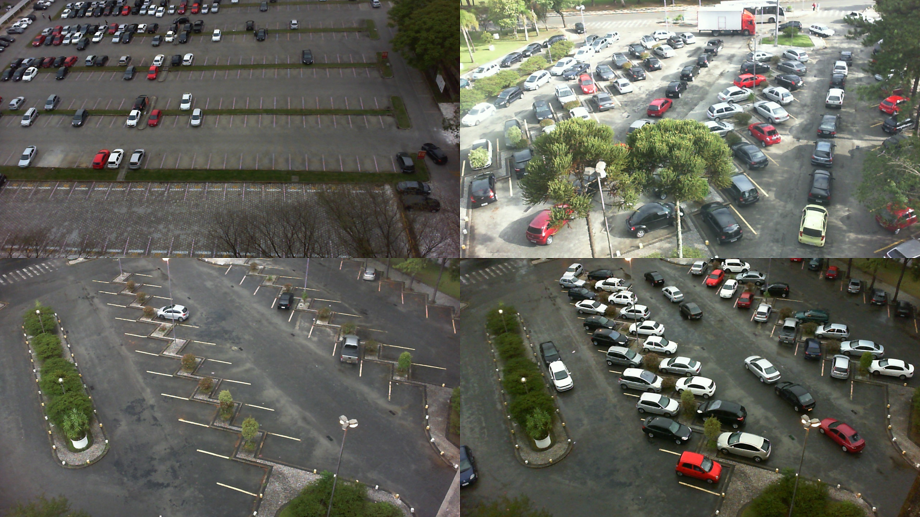
\includegraphics[width=1\textwidth]{VnVPlan/BlanderbussDataset.png}
  \end{center}
\end{figure}

\begin{figure}[h!]
  \begin{center} 
  \caption{CNRPark Dataset Sample}
  \label{CNRParkSample}
        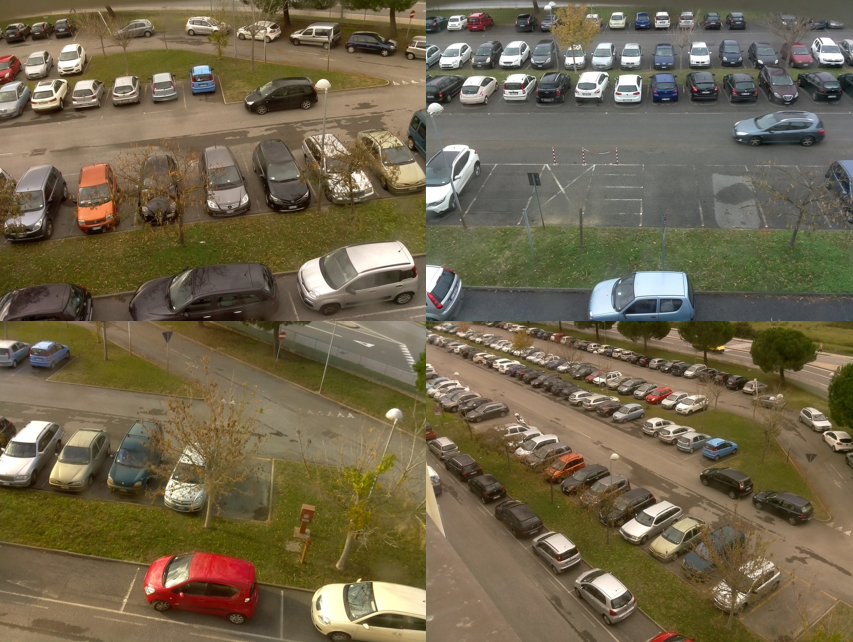
\includegraphics[width=1\textwidth]{VnVPlan/CNRParkDataset.png}
  \end{center}
\end{figure}

\clearpage

\section{System Test Description}
	
\subsection{Tests for Functional Requirements}

\wss{Subsets of the tests may be in related, so this section is divided into
  different areas.  If there are no identifiable subsets for the tests, this
  level of document structure can be removed.}

\wss{Include a blurb here to explain why the subsections below
  cover the requirements.  References to the SRS would be good here.}

\subsubsection{Area of Testing1}


\begin{table}[!h]
\begin{center}
\caption {STC\_001}
\label{tab:STC_001}
\begin{tabular}{ | m{1.5cm} | m{15cm} | } 
\hline
ID & \nameref{tab:STC_001} \\ 
\hline
Control & Manual \\ 
\hline
Initial State & The product is in its Off state. \\ 
\hline
Input & Enter the configure state and set the hover height parameters to be the smallest values possible value \ref{Min_Hover_Params}. Afterward, launch the drone in normal operation and wait for 1 min 25 sec. \\ 
\hline
Output & From the moment of launch, it should take less than 25 seconds to reach and hover within 7+-1.5 m. While hovering, the drone should laterally stay within a 1.5 m radius of the launch location, and it should stay within 5.5m and 8.5m above the ground at all times. \\ 
\hline
How the test will be performed & 
The first step of the test, configuring height parameters, is accomplished by:
\begin{enumerate}[topsep=0pt,itemsep=-1ex,partopsep=1ex,parsep=1ex]
    \item Setting the input i\_Mode as Configure and turning the power switch of the drone to On.
    \item Assert m\_Launch, so the drone enters the Configure state.
    \item Setting the height parameters in the Operator's PC Application to \ref{Min_Hover_Params}.
\end{enumerate}
The second step of the drone, having the drone enter and stay within the hover state, is accomplished by:
\begin{enumerate}[topsep=0pt,itemsep=-1ex,partopsep=1ex,parsep=1ex]
	\item Turning the power switch on the drone off.Then Setting i\_Mode as Normal and turning the power switch on, so the drone enters  Idle state.
	\item Placing the drone in a non-parking lot area. 
	\item Asserting m\_Launch as true, then wait for 25 sec.
	\item Wait for 1 min. During this wait measure the output variables.
\end{enumerate}
Once the output variables have been measured and the test is complete:
Assert m_Land to true, so that drone will enter the land state.\\ 
\hline
Test case derivation & As per SRS, the smallest possible height parameters are \ref{Min_Hover_Params}. 

As per SRS, the drone should take less than 25 seconds to reach i\_MaxHoverHeight (7+-1.5 m) from the moment the drone launches. This is why the input steps specify a 25-second wait after launch.

As per SRS, while in the Hover state, the drone will enter the Autonomous Explore state if it sees a parking lot. The purpose of placing the drone in a non-parking lot area was to keep the drone in the Hover state.

While hovering the drone should stay within a 1.5 m radius. In terms of height, it means that the drone should hover within i\_MaxHoverHeight-1.5m=7-1.5=5.5m and i\_MaxHoverHeight+1.5m=7+1.5=8.5m above the ground.  
\\ 
\hline
Purpose of test and/or relationship to other tests & This verifies the configure state can change flight parameters in accordance with the restrictions specified in the SRS. 
Elucidates how the drone operates in a non-parking lot area.
Verifies that the drone's flight dynamics are accurate, to the point that it can fly at the minimum height while maintaining minimum height safety requirements.
Verifies the states Off, Idle, Hover, Configure and Land as well as the transitions between them. In particular, it verifies NFR requiring the drone to stay within a 1.5m radius within the hover state. 
Verifies a corner case in the parking lot detection algorithm, that it correctly detects no parking lot when there is no parking lot.
Verifies the NFR requiring the product to takeoff to i\_MaxHoverHeight within 25 seconds. \\ 
\hline
\end{tabular}
\end{center}
\end{table}

\begin{table}[!h]
\begin{center}
\caption {STC\_002}
\label{tab:STC_002}
\begin{tabular}{ | m{1.5cm} | m{15cm} | } 
\hline
ID & \nameref{tab:STC_002}  \\ 
\hline
Control & Manual\\ 
\hline
Initial State & The product is in its Off state.
 \\ 
\hline
Input & Enter the configure state and set the hover height parameters to be \ref{Med_Hover_Params}. Afterward, launch the drone in normal operation wait for 1 min 25 sec. \\ 
\hline
Output & The drone should take less than 25 seconds to reach and hover within 7+-1.5 m from the moment the drone launches. While hovering, the drone should laterally stay within a 1.5 m radius of the launch location, and it should stay within 18.5m and 21.5m above the ground at all times. 
 \\ 
\hline
How test will be performed &
The first step of the test, configuring height parameters, is accomplished by:
\begin{enumerate}[topsep=0pt,itemsep=-1ex,partopsep=1ex,parsep=1ex]
    \item Setting the input i\_Mode as Configure and turning the power switch of the drone to On.
    \item Assert m\_Launch, so the drone enters the Configure state.
    \item Setting the height parameters in the Operator's PC Application to \ref{Med_Hover_Params}.
\end{enumerate}
The second step of the drone, having the drone enter and stay within the hover state, is accomplished by:
\begin{enumerate}[topsep=0pt,itemsep=-1ex,partopsep=1ex,parsep=1ex]
	\item Turning the power switch on the drone off.Then Setting i\_Mode as Normal and turning the power switch on, so the drone enters  Idle state.
	\item Placing the drone in a non-parking lot area. 
	\item Asserting m\_Launch as true, then wait for 25 sec.
	\item Wait for 1 min. During this wait measure the output variables.
\end{enumerate}
Once the output variables have been measured and the test is complete:
Assert m_Land to true, so that drone will enter the land state.\\ 
\hline
Test case derivation & As per SRS, the drone should take less then 25 seconds to reach i\_MaxHoverHeight (20+-1.5 m) from the moment the drone launches. This is why the input steps specify a 25 second wait after launch.

As per SRS, while in the Hover state, the drone will enter the Autonomous Explore state if it sees a parking lot. The purpose of placing the drone in a non-parking lot area was to keep the drone in the Hover state.

While hovering the drone should stay a 1.5 m radius. In terms of height, it means that the drone should hover within i\_MaxHoverHeight-1.5m=20-1.5=18.5m and i\_MaxHoverHeight+1.5m=20+1.5=21.5m above the ground.  \\ 
\hline
Purpose of test and/or relationship to other tests & This test is very similar to test case 1, except that the height parameters are configured to be much higher. The purpose of configuring the height parameters differently is to verify that the drone can hover accurately at different heights, that the drone can land safely from different heights, and that the Configure state is actually capable of configuring the height variables.

Verifies the states Off, Idle, Hover, Configure and Land as well as the transitions between them. In particular, it verifies NFR requiring the drone to staying within a 1.5m radius within the hover state. 
Verifies a corner case in the parking lot detection algorithm, that it correctly detects no parking lot when there is no parking lot.
Elucidates how the drone operates in a non-parking lot area.
Verifies the NFR requiring the product to takeoff to i\_MaxHoverHeight within 25 seconds. \\ 
\hline
\end{tabular}
\end{center}
\end{table}


\begin{table}[!h]
\begin{center}
\caption {STC\_003}
\label{tab:STC_003}
\begin{tabular}{ | m{3.2cm} | m{12.2cm} | } 
\hline
ID & \nameref{tab:STC_003} \\ 
\hline
Control & Manual \\ 
\hline
Initial State & The product is in the Idle state. \\ 
\hline
Input & Record the remaining battery stated on the Operator's PC Application. Disconnect the battery from the drone and connect it to the battery charger and record the remaining battery levels it detects. \\ 
\hline
Output & Battery levels stated on the Operator's Application should match the battery levels stated on the battery charger. \\ 
\hline
How test will be performed & Input section contains enough detail. \\ 
\hline
Test case derivation & As per HA, the drone should display the remaining battery on the Operator's PC Application. \\ 
\hline
Purpose of test and/or relationship to other tests & Verification that the display of the remaining battery on the Operator's PC Application is accurate. \\ 
\hline
\end{tabular}
\end{center}
\end{table}

\begin{table}[!h]
\begin{center}
\caption {STC\_004}
\label{tab:STC_004}
\begin{tabular}{ | m{3.2cm} | m{12.2cm} | } 
\hline
ID & \nameref{tab:STC_004} \\ 
\hline
Control & Manual \\ 
\hline
Initial State & The product is in its Idle state. Drone battery is fully charged. \\ 
\hline
Input & To launch the drone, assert m\_Launch as true. Let the drone operate in any flying state. \\ 
\hline
Output & Observe the battery levels displayed on the Operator’s Application fall with time. It should fly in normal operation for at least 3.5 minutes.
At some point the battery will be running very low (less then 1.5 minutes of flight left) and the drone will automatically enter the Malfunction state. In this state an error message will be logged to c\_Log, the c\_HealthStatus is set to Unhealthy, and the drone returns to the launch location. \\ 
\hline
How test will be performed & Regarding the initial state, verifying that the battery capacity is full can be accomplished by using the battery's charger. Input steps are self explanatory. \\ 
\hline
Test case derivation & As per SRS, the Malfunction state must send an error message to c\_Log, change the c\_HealthStatus is set to Unhealthy, and the drone returns to the launch location.
As per HA, the drone must enter the Malfunction state and land itself when the battery left is detected as low (less then 1.5 minutes). As per SRS, the drone must have a total battery capacity of lasting at least 5 minutes, leading to at least 3.5 minutes of flight.
As per HA, the drone must display the amount of battery remaining to the operator. 
 \\ 
\hline
Purpose of test and/or relationship to other tests & 
\begin{itemize}
    \item Verification of the low battery transition to the malfunction state. 
    \item Verification of the operation of the malfunction state and transition into it.
    \item Verification of the NFR requiring flight time to be at least 5 minutes. 
    \item Verification of the FR requiring the drone to display remaining battery life to the operator. 
\end{itemize}
\\ 
\hline
\end{tabular}
\end{center}
\end{table}

\begin{table}[!h]
\begin{center}
\caption {STC\_005}
\label{tab:STC_005}
\begin{tabular}{ | m{3.2cm} | m{12.2cm} | } 
\hline
ID & \nameref{tab:STC_005} \\ 
\hline
Control & Manual \\ 
\hline
Initial State & The product is in its Idle state. Drone has less then 3 minutes of battery remaining.  \\ 
\hline
Input & Attempt to launch the drone via setting m\_Launch as true. \\ 
\hline
Output & Drone should not launch, and instead a descriptive error should be logged into the variable c\_Log.  \\ 
\hline
How test will be performed & Input section contains enough detail. \\ 
\hline
Test case derivation & As per HA, the drone should not fly unless there is more the 3 minutes of battery remaining.
 \\ 
\hline
Purpose of test and/or relationship to other tests & Verification of the FR requiring the drone to not fly unless their sufficient battery is available. 
\\ 
\hline
\end{tabular}
\end{center}
\end{table}

\begin{table}[!h]
\begin{center}
\caption {STC\_006}
\label{tab:STC_006}
\begin{tabular}{ | m{3.2cm} | m{12.2cm} | } 
\hline
ID & \nameref{tab:STC_006} \\ 
\hline
Control & Manual \\ 
\hline
Initial State & The product is in any of its flying states.   \\ 
\hline
Input & Set m\_CompulsiveMove as false. Change m\_DesiredUserLoc to a location within the parking lot and to the diagonal front right of the drone at least 20m away.  \\ 
\hline
Output & The drone should enter the Manual Move state upon a change to m\_DesiredUserLoc. The drone should move to and stay within 1.5m radially of the specified location. 
The user should also see a visual trace of the drone's movement; it should be a roughly straight line (shortest path).
Measure the time takes to reach the specified GPS location and calculate average speed and ensure it is more then 4 m/sec.  \\ 
\hline
How test will be performed & Input section contains enough detail. \\ 
\hline
Test case derivation & As per SRS, the drone should enter Manual Move state whenever m\_DesiredUserLoc is changed and m\_CompulsiveMove is false. In this state the drone should travel to m\_DesiredUserLoc and hover with an accuracy of 1.5m. 

A visual trace of the drone's movement in the past 60 seconds should be displayed on the Operator's PC Application. It should appear as a relatively straight diagonal line toward the hover location, as the drone's path planning should make it take the shortest path. 

Using the time taken, the average speed of the drone can be calculated as distance/time. As per the SRS, it should be at least 4 m/sec. 
 \\ 
\hline
Purpose of test and/or relationship to other tests & 
\begin{itemize}
    \item Assesses the ability of the drone to move to forward as well as move rightward in a stable and efficient manner toward a specified GPS location.
    \item Helps verify the Manual Move state and transitions related to proceeding to a given location when the location is within the parking lot.
    \item Verifies the NFRs related to lateral accuracy. 
    \item Verifies the visual trace requirement. 
    \item Verifies the average speed requirement. 
\end{itemize}
\\ 
\hline
\end{tabular}
\end{center}
\end{table}

\begin{table}[!h]
\begin{center}
\caption {STC\_007}
\label{tab:STC_007}
\begin{tabular}{ | m{3.2cm} | m{12.2cm} | } 
\hline
ID & \nameref{tab:STC_007} \\ 
\hline
Control & Manual \\ 
\hline
Initial State & The product is in any of its flying states.   \\ 
\hline
Input & Set m\_CompulsiveMove as false. Change m\_DesiredUserLoc to a location outside the parking lot and in front of the drone.  \\ 
\hline
Output & The drone should enter the Manual Move State upon a change to m\_DesiredUserLoc. The drone should move forward towards the location, until it is close to the edge of the parking lot after which the drone should enter the Desired Location Error State. Upon entry to this state, it logs an error to the user in c\_Log and sets c\_UserError to Desired\_Location\_Out\_Of\_Bounds. 

There should be a straight line in the visual trace of the past GPS location if the path planning algorithm is correctly optimized to take the shortest path toward the GPS location. 

Monitor the FPS of the c\_CameraView output; it should be more then 0.5 FPS.  \\ 
\hline
How test will be performed & Input section contains enough detail. \\ 
\hline
Test case derivation & As per SRS, the drone should enter Manual Move whenever m\_DesiredUserLoc is changed and m\_CompulsiveMove is false. Given the GPS location being in front of the drone, it should fly forward, but when it recognizes that the requested GPS location is outside the parking lot, it should enter the Desired Location Error State. Within this state, the SRS specifies that the drone should inform the user that their movement command is not possible (through a message in c\_Log), and begin hovering in place.

A visual trace of the drone's movement in the past 60 seconds should be displayed on the Operator's PC Application. It should appear as a relatively straight line toward the hover location, as the drone's path planning should make it take the shortest path. 
As per SRS, the FPS should be more then 0.5.
 \\ 
\hline
Purpose of test and/or relationship to other tests & 
Assesses the ability of the drone to fly to forward.
Verifies the drone’s ability to identify Parking Lot boundaries.
Helps verify the Manual Move state and transitions related to it, specifically its ability to detect and report the error when requested location is invalid. 
Verifies the Desired Location Error state and transitions related to it. 
Verifies the visual trace requirement. 
Verifies the NFR specifying minimum required FPS of c\_CurrentView to be at least 0.5.
\\ 
\hline
\end{tabular}
\end{center}
\end{table}

\begin{table}[!h]
\begin{center}
\caption {STC\_008}
\label{tab:STC_008}
\begin{tabular}{ | m{3.2cm} | m{12.2cm} | } 
\hline
ID & \nameref{tab:STC_008} \\ 
\hline
Control & Manual \\ 
\hline
Initial State & The drone is on the ground of a rectangular shaped parking lot with less then 30 parking spots, is fully charged and is in its idle state.  \\ 
\hline
Input & Assert m\_Launch. \\ 
\hline
Output & The drone should first enter the Hover state, but once it begins hovering and it detects the parking lot, the drone should enter the Autonomous Explore state. Within the 3.5 minutes of guaranteed operations, the drone should have explored the full parking and completed its c\_OccupancyMap with reasonable accuracy. 
Monitor the FPS and output of c\_CameraView output. \\ 
\hline
How test will be performed & Input section contains enough detail. \\ 
\hline
Test case derivation & As per SRS, while in the hover state, the drone should enter the Autonomous Explore state automatically once it detects a parking lot. The Autonomous Explore state specifies that the drone should explore the parking lot during this state. Assuming that the drone moves at roughly 4m/sec and sees at least 1 parking spot every frame, it is reasonable to assume that 3.5 minutes is more then enough time for the drone to explore an entire parking lot of this size.
 \\ 
\hline
Purpose of test and/or relationship to other tests & 
\begin{itemize}
    \item Assesses the accuracy of the visual perception algorithm to segment the parking lot, accuracy in recognizing unoccupied parking spots, and accuracy in its generated occupancy map (c\_OccupancyMap).
    \item Assesses the accuracy of the path planning algorithm (does it ever explore the same area twice, does it explore the parking lot in a systematic and predictable way, etc.).
    \item Verifies the drone’s ability to identify Parking Lot boundaries.
    \item Helps to verify the Autonomous explore state as well as the transition to it from the Hover state.
    \item Verifies the NFR specifying minimum required FPS of c\_CurrentView to be 0.5.
    \item Verifies the NFR requiring that the drone explores up to 1400m\^2 of the parking lot assuming enough time and small enough size of the parking lot.
\end{itemize}
\\ 
\hline
\end{tabular}
\end{center}
\end{table}

\begin{table}[!h]
\begin{center}
\caption {STC\_009}
\label{tab:STC_009}
\begin{tabular}{ | m{1.5cm} | m{15cm} | } 
\hline
ID & \nameref{tab:STC_009} \\ 
\hline
Control & Manual \\ 
\hline
Initial State & The height parameters are set as \ref{Min_Hover_Params}. The drone is in the Hover state, on the surface of a non-parking lot area but atleast 50m away from a parking lot.  \\ 
\hline
Input & Attempt to enter the Autonomous Explore state. Now move the drone to a location within the nearby parking lot utilizing the Compulsive Move state. Once the drone is in the parking lot attempt to enter the Autonomous Explore State again. \\ 
\hline
Output & Upon the first attempt to enter the Autonomous Explore State, the attempt should fail, and instead the drone should enter the No Parking Lot Detected State. Upon entrance to this state, c_UserError is set to No_Lot_Detected_State and an error message is logged to c_Log. Afterward, when the drone enters the Compulsive move state, c_UserError should be None, and the drone should travel to m_DesiredUserLoc. Upon the second attempt to enter the Autonomous Explore State, the attempt should succeed. \\ 
\hline
How test will be performed & 
The test case can be restated in terms of the input and output variables: 
\begin{enumerate}[topsep=0pt,itemsep=-1ex,partopsep=1ex,parsep=1ex]
	\item Assert m_AutonomousExplore as true to request the Autonomous Explore state. Measure/analyze behavior. 
	\item Now assert and hold m_CompulsiveMove as true, and change m_DesiredUserLoc to a location within the nearby parking lot. 
	\item Wait until the drone is within 1.5m of the m_DesiredUserLoc
	\item Try setting m_AutonomousExplore to true again to request entrance in the parking lot. Measure/analyze behavior.  \end{enumerate} \\
\hline
Test case derivation & As per SRS the Autonomous Explore state should only be entered if c_ParkingLotDetected is true. The Initial State behaviour specified above (height parameters and distance to nearby parking lot) are set in a way to ensure that the nearby parking lot is not in the field of view of the drone. This is why the first attempt to enter the Autonomous Explore fails while the second attempt succeeds. When an attempt to enter Autonomous Explore fails, the drone should enter the No Parking Lot Detected State.

As per SRS, upon entrance into the No Parking Lot Detected State c_UserError should be set to No_Lot_Detected_State and an error message is should be logged to c_Log. Upon exit c_UserError should be set to None.

As per SRS the Compulsive Move state should be entered if the m_DesiredUserLoc is changed and m_CompulsiveMove is true. 
 \\ 
\hline
Purpose of test and/or relationship to other tests & 
\begin{itemize}
    \item Not that although there is a requirement regarding how the drone should move to m_DesiredUserLoc with 1.5m of accuracy within Compulsive Move, it is not verified in this testcase. The reason is that because the drone moves such long distances and it never actually hovers at m_DesiredUserLoc (as it transitions to Autonomous Explore), it makes measuring GPS location of the drone difficult.
    \item Assesses the accuracy of the visual perception algorithm in recognizing parking lot area. 
    \item Helps to verify the Autonomous explore state as well as the transition to it from the input m_AutonomousExplore. 
    \item Verifies the Compulsive Move state as well as transitions related to it.
    \item Verifies the No Parking Lot Detected Error state as well as transitions related to it.
\end{itemize}
\\ 
\hline
\end{tabular}
\end{center}
\end{table}
\subsection{Tests for Nonfunctional Requirements}

\wss{The nonfunctional requirements for accuracy will likely just reference the
  appropriate functional tests from above.  The test cases should mention
  reporting the relative error for these tests.  Not all projects will
  necessarily have nonfunctional requirements related to accuracy}

\wss{Tests related to usability could include conducting a usability test and
  survey.  The survey will be in the Appendix.}

\wss{Static tests, review, inspections, and walkthroughs, will not follow the
format for the tests given below.}

\subsubsection{Area of Testing1}
		
\paragraph{Title for Test}

\subsubsection{Area of Testing2}

...

\subsection{Traceability Between Test Cases and Requirements}

\wss{Provide a table that shows which test cases are supporting which
  requirements.}

\section{Unit Test Description}

\wss{Reference your MIS (detailed design document) and explain your overall
  philosophy for test case selection.}  
\wss{This section should not be filled in until after the MIS (detailed design
  document) has been completed.}

\subsection{Unit Testing Scope}

\wss{What modules are outside of the scope?  If there are modules that are
  developed by someone else, then you would say here if you aren't planning on
  verifying them.  There may also be modules that are part of your software, but
  have a lower priority for verification than others.  If this is the case,
  explain your rationale for the ranking of module importance.}

\subsection{Tests for Functional Requirements}

\wss{Most of the verification will be through automated unit testing.  If
  appropriate specific modules can be verified by a non-testing based
  technique.  That can also be documented in this section.}

\subsubsection{Module 1}

\wss{Include a blurb here to explain why the subsections below cover the module.
  References to the MIS would be good.  You will want tests from a black box
  perspective and from a white box perspective.  Explain to the reader how the
  tests were selected.}

\item{test-id1\\}

Type: \wss{Functional, Dynamic, Manual, Automatic, Static etc. Most will
  be automatic}		
Initial State: 				
Input: 
					
Output: \wss{The expected result for the given inputs}

Test Case Derivation: \wss{Justify the expected value given in the Output field}

How test will be performed: 
					
\item{test-id2\\}

Type: \wss{Functional, Dynamic, Manual, Automatic, Static etc. Most will
  be automatic}
					
Initial State: 
					
Input: 
					
Output: \wss{The expected result for the given inputs}

Test Case Derivation: \wss{Justify the expected value given in the Output field}

How test will be performed: 

\item{...\\}
    
\subsubsection{Module 2}

...

\subsection{Tests for Nonfunctional Requirements}

\wss{If there is a module that needs to be independently assessed for
  performance, those test cases can go here.  In some projects, planning for
  nonfunctional tests of units will not be that relevant.}

\wss{These tests may involve collecting performance data from previously
  mentioned functional tests.}

\subsubsection{Module ?}
		
\begin{enumerate}

\item{test-id1\\}

Type: \wss{Functional, Dynamic, Manual, Automatic, Static etc. Most will
  be automatic}
					
Initial State: 
					
Input/Condition: 
					
Output/Result: 
					
How test will be performed: 
					
\item{test-id2\\}

Type: Functional, Dynamic, Manual, Static etc.
					
Initial State: 
					
Input: 
					
Output: 
					
How test will be performed: 

\end{enumerate}

\subsubsection{Module ?}

...

\subsection{Traceability Between Test Cases and Modules}

\wss{Provide evidence that all of the modules have been considered.}
				
\bibliographystyle{plainnat}

\bibliography{../../refs/References}

\newpage

\section{Appendix}

This is where you can place additional information.

\subsection{Symbolic Parameters}

The definition of the test cases will call for SYMBOLIC\_CONSTANTS.
Their values are defined in this section for easy maintenance.

\MakeRobust{\ref}% avoid expanding it when in a textual label

\makeatletter
\newcommand{\labeltext}[2]{%
  \@bsphack
  \csname phantomsection\endcsname % in case hyperref is used
  \def\@currentlabel{#1}{\label{#2}}%
  \@esphack
}
\makeatother
\begin{table}[!h]
\begin{center}
\caption {Symbolic Constants}
\label{tab:symbolic_constants}
\begin{tabular}{ | m{5cm} | m{8cm} | } 
\hline
ID & \nameref{tab:symbolic_constants} \\ 
\hline
Min_Hover_Params\labeltext{Min_Hover_Params}{Min_Hover_Params} & (i\_MinHoverHeight=7, i\_-MaxHoverHeight=7, i\_DesiredHoverHeight=7) \\ 
\hline
Med_Hover_Params\labeltext{Med_Hover_Params}{Med_Hover_Params} & (i\_MinHoverHeight=20, i\_-MaxHoverHeight=20, i\_DesiredHoverHeight=20) \\ 
\hline
\end{tabular}
\end{center}
\end{table}
\subsection{Usability Survey Questions?}
\wss{This is a section that would be appropriate for some projects.}

\newpage{}
\section{Appendix --- Reflection}
This section reviews the roles mentioned in Table \ref{VnV_Team} and evaluates each team member on the graduate attribute of Lifelong Learning. 

  
\begin{table}[!h]
\begin{center}
\caption {Required Testing}
\label{RequiredTesting}
\begin{tabular}{ | m{3cm} | m{3cm} | m{8cm} | }
\hline
Test & Responsibility & Rationale\\
\hline
Dynamic Testing & Fady, Muhammad, Zaid \& Winnie & Dynamic testing is vital, especially for flying a drone. Dynamic testing is executing test cases in variable environments to analyze how the system behaves.\\
\hline
Integration Testing & Muhammad & Integration testing is important as it will test different units, modules, or components of the drone as a combined entity.\\
\hline
Static Testing & Fady, Muhammad \& Winnie & Static testing involves matching the requirements from the SRS to the code written. Static testing also involves looking into code format and errors. \\
\hline
 Visual Perception and Path Planning Testing & Fady & Verifies that the visual perception and autonomous exploration algorithm is performing within specifications. \\
\hline
Drone Finite State Machine (FSM) and Communication Testing & Ali & Verifies that all communication between the drone components and the drone to the Operator's application is working correctly. \\
\hline
Mechanical Testing & Zaid & Verifies that all physical components and the dynamics are working within specifications. \\
\hline
Operator's Application Testing & Winnie & Verifies that the Operator's application and user manual meet the specifications outlined.
\\
\hline
\end{tabular}
\end{center}
\end{table}

\subsection{Knowledge & Skills}
Table \ref{KnowledgeTable} covers different approaches to follow the plan from Table \ref{RequiredTesting}.

\begin{table}[!h]
\begin{center}
\caption {Knowledge Acquisition}
\label{KnowledgeTable}

\begin{tabular}{ | m{3cm} | m{7cm} | m{4cm} | }

\hline
Test & Approaches & Verdict \\
\hline
Dynamic Testing & 
Approach 1: Previous lecture notes from McMaster's MECHTRON 3K04: Software Development. \newline Approach 2: Research online and watch tutorials such as \href{https://www.youtube.com/watch?v=ePMjdL4PE5M}{this video} on YouTube.\newline Approach 3: Research online and find resources for mechanical static testing such as \href{https://www.sciencedirect.com/topics/materials-science/dynamic-mechanical-analysis}{this}.& Fady, Muhammad \& Winnie will proceed with Approach 2 as MECHTRON 3K04 did not go in-depth with Static Testing. Zaid will proceed with Approach 3 for Mechanical Testing.  \\
\hline
Integration Testing & 
Approach 1: Previous lecture notes from McMaster's MECHTRON 3K04: Software Development. \newline Approach 2: Research online resources such as \href{https://www.simplexitypd.com/blog/five-tips-for-mechatronic-system-integration}{this website}. & Muhammad will proceed with Approach 2 to get more knowledge with Integration Testing as the MECHTRON 3K04 course did not get in-depth with the subject. \\
\hline
Static Testing & 
Approach 1: Previous lecture notes from McMaster's MECHTRON 3K04: Software Development \newline Approach 2: Research online and find resources for static testing such as \href{https://www.guru99.com/testing-review.html}{this website}. & Fady, Muhammad \& Winnie will proceed with Approach 1 as Static Testing was done extensively in the MECHTRON 3K04 Pacemaker project.\\
\hline
 Visual Perception and Path Planning Testing & Approach 1: Watch McMaster's Google Developer's Club \href{https://www.youtube.com/watch?v=Zrw5eCfnSOM}{video} on YouTube to learn more about the OpenCV library complementing ENG 1D04: Engineering Computation.  \newline Approach 2: Use OpenCV \href{https://docs.opencv.org/4.x/d9/df8/tutorial_root.html}{tutorial documentation}. & Fady will proceed with Approach 1 as the tutorial was done at McMaster by McMaster students going through the fundamentals of OpenCV.\\
\hline
Drone Finite State Machine (FSM) and Communication Testing & 
Approach 1: Previous lecture notes from McMaster's MECHTRON 3K04: Software Development \newline Approach 2: Use \href{http://wiki.ros.org/smach}{ROS.org documentation} on ROS' library SMACH to learn more about the FSM implementation. & Muhammad will proceed with Approach 2 to get familiar with the SMACH library which will be more relevant for drone development.\\
\hline
\end{tabular}
\end{center}
\end{table}

  
\begin{table}[!h]
\begin{center}
\label{RequiredTesting}

\begin{tabular}{ | m{3cm} | m{7cm} | m{4cm} | }

\hline
Test & Approaches & Verdict \\

\hline
Mechanical Testing & Approach 1: Previous lecture notes from McMaster's ENG 1C03: Engineering Design \& Graphics \newline Approach 2: Watch \href{https://www.youtube.com/watch?v=YmMDhzXitn0}{SolidWorks' basic tutorial}.& Zaid will use Approach 2 to get familiar with SolidWorks.\\  
\hline
Operator's Application Testing & Previous lecture notes from McMaster's MECHTRON 1D04: Engineering Computation  to understand the language of the application. \newline Approach 2: Use \href{https://docs.python.org/3/tutorial/}{Python Documentation} and other online resources to understand Python syntax. & Winnie will proceed with Approach 1 as ENG 1D04 had covered Python extensively.\\
\hline


\end{tabular}
\end{center}
\end{table}

\end{document}